% 国赛 (CUMCM) 模板
% 基于 cumcmthesis 文档类
% 电子版提交使用 withoutpreface 去掉封面编号页，bwprint 黑白打印
\documentclass[withoutpreface,bwprint]{cumcmthesis}

% === 额外宏包（cumcmthesis 已内置 amsmath/graphicx/booktabs/listings/hyperref/tabularx/longtable 等）===
\usepackage[framemethod=TikZ]{mdframed}
\usepackage[section]{placeins}
\usepackage{needspace}

% === 参考文献引用（数字型，配合 gbt7714-numerical.bst）===
%  不要额外加载 cite 宏包，以免和 natbib 冲突。
%  必须显式加载 natbib：gbt7714-numerical.bst 产出的是 natbib 风格条目
%    （\bibitem[作者(年)]{key}），不加载 natbib 时标准 \cite 会把"作者-年"当引用标记
%    上标出来（而非数字 [1]）。numbers 模式让 \cite 产出数字，cls 的 \upcite 再上标它。
%    正文引用统一用 \upcite{key} 得数字上标 $^{[1]}$。
\usepackage[numbers,sort&compress]{natbib}

% === TikZ（cumcmthesis 已加载 tikz，这里只加额外库）===
\usetikzlibrary{arrows.meta,positioning,shapes.geometric,fit,calc}

% === 代码高亮设置 ===
\lstset{
    language=Python,
    basicstyle=\small\ttfamily,
    breaklines=true,
    breakatwhitespace=false,
    columns=fullflexible,
    keepspaces=true,
    frame=single,
    numbers=left,
    numberstyle=\tiny,
    literate={λ}{{$\lambda$}}1,
}

% === 摘要后排版修复 ===
%  不再重定义 \@cite —— 引用交给 natbib（上面已 numbers 模式加载），
%    \upcite 会正确产出数字上标；旧的 \@cite hack 在 natbib 下无效且会干扰，已移除。
\makeatletter
% === 修复摘要后排版（cls 的 abstract 结束时有 \newpage\null，跟目录前的 \newpage 冲突产生空白页）===
% 方案：abstract 结束时加 \newpage 确保目录另起一页，但不加 \null 避免空白页
\renewenvironment{abstract}{%
  \if@twocolumn\section*{\abstractname}%
  \else\begin{center}{\zihao{4}\bfseries \abstractname\vspace{-.5em}\vspace{\z@}}\end{center}\quotation
  \fi}{\if@twocolumn\else\endquotation\newpage\fi}
\makeatother

% === 竞赛信息（电子版提交时注释掉）===
% \tihao{A}
% \baominghao{xxxx}
% \schoolname{}
% \membera{}
% \memberb{}
% \memberc{}
% \supervisor{}
% \yearinput{}
% \monthinput{}
% \dayinput{}

\title{基于时序学习与整数规划的世界杯观赛需求及资源协同优化}

% MH-FLOAT-TUNE 受控浮动调参（防整页空白/一页一图）
% placeins 已由模板/cls 加载，此处不重复注入（避免 Option clash）
\renewcommand{\topfraction}{0.92}
\renewcommand{\bottomfraction}{0.9}
\renewcommand{\textfraction}{0.06}
\renewcommand{\floatpagefraction}{0.72}
\renewcommand{\dbltopfraction}{0.92}
\renewcommand{\dblfloatpagefraction}{0.72}
\setcounter{topnumber}{3}
\setcounter{bottomnumber}{2}
\setcounter{totalnumber}{4}
\begin{document}

\maketitle

% === 摘要 ===
\begin{abstract}

世界杯赛事安排同时连接观赛需求、竞技公平、场馆能力、跨城旅行与赛中资源保障。本文以题目附件、公开赛前信息和可核验的真实赛程为基础，构建“需求预测—联合排程—动态调配—现实比较”的闭环框架；全流程区分赛前、赛中与赛后信息截面，并对输出进行约束复算和敏感性检验。

问题一审计 $55$ 个候选字段的时间血缘，剔除 $10$ 个同场赛后字段并主动舍弃中立场标记，在 $560$ 条训练样本内进行扩窗五折验证，再对 $140$ 条标签未知的时间外样本预测。\textbf{Elastic Net} 在当前四类候选中取得最低误差，五折平均 MSE 为 $220.0855$、\textbf{平均 RMSE 为 $14.8121$}、平均 MAE 为 $11.8276$；生成的 $72$ 场需求预测均值为 \textbf{$170321280$ 人次}。问题二以 $85680$ 个三维布尔变量建立 \textbf{CP-SAT} 联合模型，并用全部候选三元组的确定性包络完成 Min--Max，求得 \textbf{$Z_2=0.484946$}；三个独立进程跨 Python 3.11/3.12 生成逐字节相同的正式赛程。复算表明 $72$ 场唯一指派，\textbf{最小休息为 $63$ 小时}，场馆负荷为 $2$--$8$ 场，全部硬约束无违反，证书间隙约 $0.41\%$。

问题三用 \textbf{$20000$ 组联合蒙特卡洛情景}同时模拟 $24$ 场第三轮，保证每次晋级质量为 $32$；五个随机种子下晋级概率标准差最大为 $0.00469$。日预算约束下，动态目标由锁定静态方案同界重评的 $6.572230$ 提高至 \textbf{$Z_3=6.637484$}，仅 \textbf{$8/24$ 场改变配置}；五种子完整重优化的增益为 $0.065123$--$0.065434$，动态决策完全一致。问题四复核 $2022$ 年世界杯 $48$ 场小组赛，构建 \textbf{可观测结构与题内代理双层评价}：实际与优化方案的最小休息分别为 $87$ 和 $63$ 小时，场均转场距离为 $18.9868$ 和 $2019.1075$ 公里；同构代理旅行指标 $D$ 分别为 $0.213022$ 和 $0.201797$。共同 Min--Max 边界下的条件性代理总分为 $0.277058$ 与 $0.480778$，16 组权重扰动均保持优化方向；由于真实合同与运营成本仍不可观测，本文只把该总分解释为题内映射下的条件性结果。

模型的优势在于时间边界清晰、预测与优化接口统一、约束可独立复算，并能在共享状态下比较静态与动态决策；局限主要来自高观看尾部样本不足、题定旅行口径和现实运营字段缺失。该框架可推广至其他分组赛事、职业联赛和大型活动，但结论强度必须服从数据与代理的证据边界。

\keywords{时序交叉验证\quad Elastic Net\quad CP-SAT\quad 多目标优化\quad 联合蒙特卡洛\quad 动态资源配置\quad 敏感性分析\quad 最近邻代理\quad 世界杯赛程}
\end{abstract}

% 竞赛正文直接进入问题重述；完整章节结构由节标题呈现，避免目录占用篇幅。

% === 正文 ===
\section{问题重述}

\subsection{研究背景}

世界杯小组赛的组织并非单一的赛程排列问题。赛事关注度决定转播与票务需求，比赛安排又同时受到场馆容量、时区、球队休息、安保能力和转播资源的约束；进入比赛阶段以后，前两轮赛果还会改变第三轮的晋级形势、需求强度与风险水平。因此，组织者真正需要的是一条从赛前预测延伸到赛中调整、并能够与现实赛程比较的完整决策链。

题目给出由48支球队、12个小组和72场比赛构成的模拟世界杯。每组4队进行单循环赛，每队参加3场；每组前2名直接晋级，12个第三名中排名靠前的8队补足32强。候选资源包括16个场馆和80个参考时段，赛程必须满足唯一指派、相邻两轮至少60小时、场馆逐日与总负荷、黄金时段公平、安保资格以及同一时段转播容量等规则。

\subsection{四个子问题}

问题一要求在题定时间划分下预测转播观看人数。训练集560场、测试集140场，测试标签不可用于任何训练或调参；对历史赛后信息只能构造严格滞后的赛前统计。模型既要输出测试集百万人尺度预测，也要为72场模拟小组赛给出人尺度预测，从而为后续传播价值计算提供输入。

问题二需要同时确定每场比赛的场馆和开球时段。优化对象不是先选场馆、再向空闲时段填充，而是比赛、场馆、时段的联合指派；目标综合票务、传播、悬念、吸引力、成本、旅行、公平与风险八个维度。除给出综合目标值外，最终方案还须逐项通过赛程规则复算，才能称为可执行排程。

问题三固定问题二得到的第三轮场馆与时段，仅根据前两轮反馈重新配置转播优先级、安保等级、交通保障和票价。24场第三轮比赛共享同一信息截面，并在20,000次联合比分模拟中统一处理组内排名与跨组第三名竞争。动态方案需与赛前已经优化并锁定的静态方案在相同动作域、相同日约束和相同归一化边界下比较，以识别信息更新带来的真实增益。

问题四选取一届已结束的四队小组制世界杯，将实际小组赛与本文72场优化方案放入同一评价函数。由于两项赛事分别有48场和72场，票务、传播、成本、旅行与风险等总量必须先转换为场均强度。现实数据中的商业和安保字段无法直接观测时，应把代理指标与可观测结构分层报告，不用代理综合分数替代对现实组织约束的判断。

\subsection{总体研究路线}

四问之间存在明确的输入输出关系：问题一提供赛前观看需求，问题二把需求转化为场馆时段排程；问题三读取该排程的第三轮部分，问题四则复用问题二的评价口径。围绕这条链路，本文先冻结数据与单位口径，再进行预测、联合优化、动态重配置和现实比较，最后统一开展约束审计与敏感性检验。整体步骤及各阶段交付见图\ref{fig:roadmap}。

\begin{figure}[htbp]
\centering
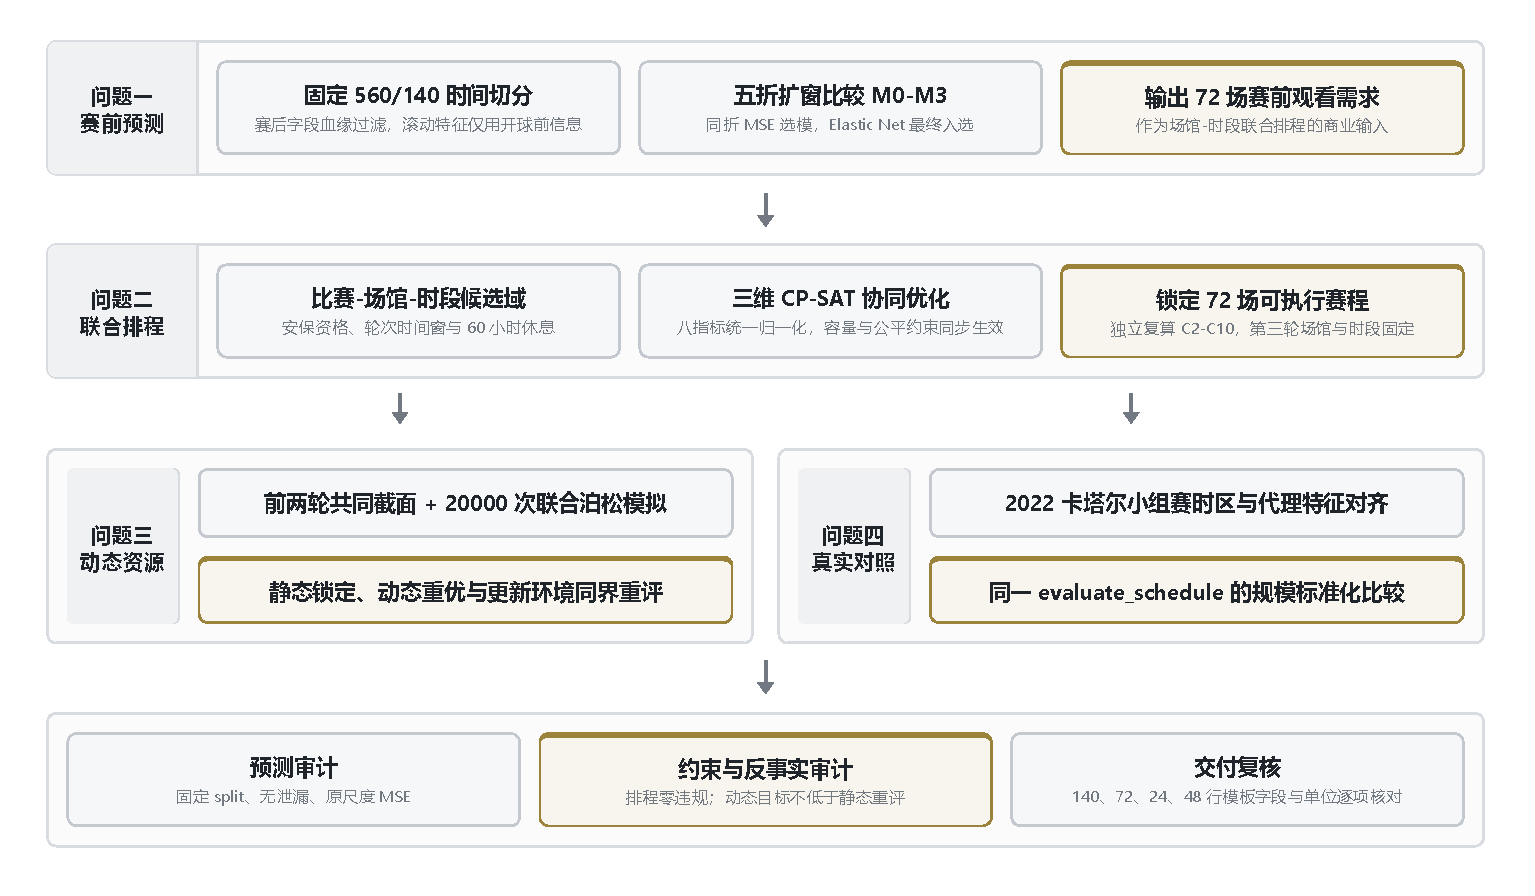
\includegraphics[width=0.85\textwidth,height=0.7\textheight,keepaspectratio]{../figures/fig_roadmap.pdf}
\caption{整体技术路线图}\label{fig:roadmap}
\end{figure}

数据合同与约束审计贯穿全部四问，而不是仅在求解结束后补做检查（见图\ref{fig:roadmap}）。预测结果以两种单位导出，排程结果以72行物理方案保存，动态策略以24场动作保存，实际赛程以48行长表保存；这种逐层固化使后续模型能够直接追溯上游输入。最终评价只复用已经定义的指标和方向，避免为迎合某个方案而重新选择分母或归一化边界。

\section{问题分析}

\subsection{信息边界与预测任务}

观看需求受球队实力、比赛阶段、球迷基础、悬念和时区共同影响\upcite{borland_2003_sport_demand}，但附件还含有同场进球、射门、上座和观看人数等赛后字段。若把这些字段直接送入模型，验证误差虽会下降，模型却无法在开球前使用。因此，问题一先审计字段的可获得时刻，再讨论回归精度。训练记录按日期排序；同一日期的比赛先生成特征，日末才更新球队历史，验证窗的观看标签在特征重建前整段屏蔽。

模型比较采用五折扩窗验证，每一验证窗都晚于训练窗。该设计比随机划分更接近“用过去预测未来”的部署过程\upcite{bergmeir_2018_time_series_cv}。候选集包括均值基线、Elastic Net、ExtraTrees 和 CatBoost，分别覆盖线性正则化、随机树集成与有序提升\upcite{zou_2005_elastic_net,geurts_2006_extremely_randomized_trees,prokhorenkova_2018_catboost}；四类模型使用相同的训练窗和唯一选模指标 MSE，复杂模型只有在时间外证据更好时才入选。

\subsection{联合排程与动态调配}

问题二同时决定 $72$ 场比赛的场馆和开球时段。当地日负荷随时区变化，球队休息、安保资格、黄金时段公平和日级资源容量又彼此耦合；若先选场馆再排时段，第一阶段可能提前耗尽第二阶段所需的可行组合。本文以三维布尔变量统一表达比赛、场馆与时段，采用 CP-SAT 求解\upcite{rasmussen_2008_round_robin_scheduling,perron_2023_cp_sat_lp}。求解分为可行基线、辅助边界和加权主模型，三个阶段共享同一硬可行域。

票务、传播和成本在硬可行域内求统一边界，并按
\begin{equation}
\operatorname{norm}(x;x_{\min},x_{\max})=
\frac{x-x_{\min}}{x_{\max}-x_{\min}}
\end{equation}
缩放。收益项正向进入目标，成本、旅行、公平损失和风险以负号进入；已无量纲的指标不重复缩放。辅助极值若只得到带证书的上下界，主模型使用其保守包络，不能拿主方案自身反标归一化范围。

问题三固定问题二给出的第三轮场馆与时段，在第二轮结束的共同信息截面上更新球队状态。每个蒙特卡洛样本同时生成 $24$ 场比分，再统一完成 $12$ 个小组排序和最佳第三名分配；逐场独立计算会遗漏跨组名额竞争。泊松强度遵循题定更新式\upcite{dixon_1997_football_scores}，$20000$ 个联合样本估计晋级概率及条件风险\upcite{kroese_2014_monte_carlo}。随后枚举每场可行资源动作，由日级多选择整数规划在预算和等级上限内每场选一个动作；票价利用单调性取解析上界，不另设粗网格。

\subsection{同口径比较与误差传播}

问题四把可观测结构与题内代理分开。休息、跨时区、场馆日和实际旅行距离由逐场赛程直接计算；现实赛程缺失的票务、传播、成本和安保字段才使用最近邻代理。实际方案、优化方案和代理扰动场景共同确定一次 Min--Max 包络，随后复用同一评价函数。该做法避免分别归一化制造优势，也符合复合指标应公开方向、权重和敏感性的要求\upcite{oecd_2008_composite_indicators}。

四问的误差不会无条件向下游扩散。问题一的需求误差会改变问题二的软目标排序，却不改变唯一指派、容量、安保和休息等硬约束；问题二的第三轮赛程一旦锁定，问题三只能重配资源，不能借新信息改排比赛；问题四的代理只服务于现实比较，不回写前三问。相应地，灵敏度分析分别检验时间外误差、排程权重、状态参数和代理映射，并按各自影响范围解释结果。

\subsection{接口与验证合同}

表\ref{tab:interfaces}概括四问的输入输出和独立验收条件。数据事实、同域模型比较和代理情景属于不同证据层：前者可以直接陈述，第二类必须注明候选域与评价函数，代理综合分只能解释为给定映射下的条件性结果。

{\small
\setlength{\tabcolsep}{4pt}
\begin{table}[htbp]
\centering
\caption{四问接口与独立验收条件}
\label{tab:interfaces}
\begin{tabularx}{\textwidth}{c>{\raggedright\arraybackslash}X>{\raggedright\arraybackslash}X>{\raggedright\arraybackslash}X}
\toprule
问题 & 输入边界 & 输出接口 & 独立验收 \\
\midrule
一 & 开球前字段与严格滞后历史 & $140$ 条测试预测、$72$ 场需求 & 主键、行数、单位、有限正值与扩窗误差 \\
二 & 赛前需求、题定候选域与资源规则 & 比赛--场馆--时段长表 & 唯一指派、UTC 冲突、休息、容量、安保、日负荷与公平 \\
三 & 固定第三轮赛程及第二轮后共同状态 & $24$ 场动态资源动作 & 每样本 $32$ 个晋级名额、日预算、资源上限及动态不劣于静态 \\
四 & 真实逐场记录与显式代理映射 & 结构指标和条件性综合分 & 单位、方向、共同分母、共同边界与代理标记 \\
\bottomrule
\end{tabularx}
\end{table}
}

任一硬验收失败都应回到相应数据或模型接口重算。求解器状态、图形外观或补充说明不能覆盖物理不可行或信息越界。

\section{模型假设}

表\ref{tab:assumptions}只列求解所必需、而题目未直接给定的边界。每项假设都对应程序口径和失效条件；新证据若越过这些条件，必须重算相关模型，不能只修改文字解释。

{\small
\setlength{\tabcolsep}{4pt}
\renewcommand{\arraystretch}{1.08}
\begin{longtable}{p{0.15\textwidth}>{\raggedright\arraybackslash}p{0.49\textwidth}>{\raggedright\arraybackslash}p{0.25\textwidth}}
\caption{模型假设、固定口径与失效处理}\label{tab:assumptions}\\
\toprule
对象 & 固定口径 & 失效时的处理 \\
\midrule
\endfirsthead
\multicolumn{3}{c}{续表\thetable}\\
\toprule
对象 & 固定口径 & 失效时的处理 \\
\midrule
\endhead
\midrule
\multicolumn{3}{r}{续下页}\\
\endfoot
\bottomrule
\endlastfoot
预测信息集 & $560/140$ 条记录构成时间外边界；测试标签不参与训练、调参、早停或缺失值统计。同场赛后字段只可进入严格滞后的球队历史，同日比赛在日末统一更新。内部以百万人拟合，正式赛程需求再乘 $10^6$ 转为人。 & 字段获得时间晚于开球、验证窗标签进入滞后量或单位不一致时，重新构造特征并完成扩窗验证。 \\
\addlinespace
联合排程域 & 比赛、场馆和时段是一个联合决策。当地日期由 UTC 转换；第二、三轮旅行以上一轮全部安保合格候选场馆为起点取均值，遵守题定口径。归一化边界来自同一硬可行域；未证最优的辅助问题采用 incumbent 与 best bound 的保守包络。 & 只有题方更改旅行定义、候选场馆或硬约束时才重建域；不得把现实中未提供的禁用日或合同条件暗设为硬约束。 \\
\addlinespace
第三轮状态 & $24$ 场共享第二轮结束后的同一状态截面。每个样本联合生成全部比分并统一排名，跨线同分块按比例分配，使晋级名额质量恒为 $32$；更新后的泊松均值截断在 $[0.15,4.50]$。 & 若状态边界长期饱和，应重估状态函数；增加模拟次数不能修复参数错配。逐场滚动更新只能作为另一个情景。 \\
\addlinespace
静态与动态方案 & 静态动作按赛前信息优化后锁定；动态动作只在更新环境中重选资源。两者使用共同动作域、价格边界、归一化边界和日预算，因此动态最优值不得低于锁定静态值。$-1<\varepsilon_i<0$ 时票价取解析右端点。 & 若出现 $\varepsilon_i\leq-1$，票价改用有界一维搜索；同界下动态值更低则说明实现或接口错误。 \\
\addlinespace
现实比较 & $2022$ 赛程取自保存的 OpenFootball 记录并按 FIFA 页面核验，球队实力使用开赛前完整 Elo 快照。小时、公里、场馆日等结构量直接复算；商业、成本和安保缺失量仅在题内最近邻代理层使用。 & 代理集中或邻居替换只降低综合分的证据强度，不能改写结构事实；补齐真实运营数据后须重做代理层。 \\
\addlinespace
随机性与复现 & 主种子为 $20260813$，晋级模拟一次生成 $20000\times24$ 样本；CP-SAT 单线程运行，正式 CSV 再由独立程序复算硬约束。 & 样本名额不守恒、硬约束失败或不同环境输出不一致时，停止解释结果并回查数据与求解接口。 \\
\end{longtable}
}

这些假设不把未知事实伪装成观测。题定口径用于主模型，现实缺失量保留代理标记；因此论文中的结论强度始终受数据来源和可复算范围约束。

\section{符号说明}

为避免四问之间同名量混淆，表\ref{tab:symbols}同时给出单位和主要取值范围。问题四的实际场馆旅行记为 $d^{\mathrm{path}}$，问题二候选域中的复合旅行仍记为 $D$，二者不共用定义。

{\small
\setlength{\tabcolsep}{4pt}
\begin{longtable}{>{\centering\arraybackslash}p{0.19\textwidth}>{\raggedright\arraybackslash}p{0.42\textwidth}>{\centering\arraybackslash}p{0.10\textwidth}>{\centering\arraybackslash}p{0.16\textwidth}}
\caption{主要符号、单位与取值范围}\label{tab:symbols} \\
\toprule
符号 & 含义 & 单位 & 范围 \\
\midrule
\endfirsthead
\multicolumn{4}{c}{续表\thetable} \\
\toprule
符号 & 含义 & 单位 & 范围 \\
\midrule
\endhead
\midrule
\multicolumn{4}{r}{续下页} \\
\endfoot
\bottomrule
\endlastfoot
$j$ & 历史预测样本索引 & -- & $1,\ldots,700$ \\
$i$ & 模拟赛事比赛索引 & -- & $1,\ldots,72$ \\
$i\in\mathcal I_3$ & 第三轮比赛索引 & -- & $24$场 \\
$t,g,v,s,d$ & 球队、小组、场馆、时段与日期索引 & -- & \shortstack{$48/12/16$\\$80/20$} \\
$\mathcal D_{tr},\mathcal D_{te}$ & 题定训练集与测试集索引 & -- & $560,140$ \\
$Y_j,\widehat Y_j$ & 真实与预测转播观看人数 & 百万人 & $>0$ \\
$X_j(t^-)$ & 开球前可获得的特征向量 & 混合 & 训练折决定 \\
$\mathcal H_t^-$ & 球队在当前开球日前的历史信息集 & -- & 严格滞后 \\
$\alpha,\rho$ & Elastic Net惩罚强度与一范数占比 & -- & $>0,[0,1]$ \\
$e_j$ & 时间外预测残差 $Y_j-\widehat Y_j$ & 百万人 & 有限 \\
$x_{ivs}$ & 比赛$i$是否指派到场馆$v$和时段$s$ & 0--1 & $\{0,1\}$ \\
$y_v$ & 场馆$v$是否至少启用一次 & 0--1 & $\{0,1\}$ \\
$K_v$ & 场馆$v$容量 & 人 & $45500$--$94000$ \\
$\tau_s$ & 时段$s$的UTC开球时刻 & 小时 & 题定时段 \\
$L_i^{req}$ & 比赛$i$的最低安保需求等级 & 等级 & $1$--$4$ \\
$L_v^{sec}$ & 场馆$v$的安保能力等级 & 等级 & $2$--$4$ \\
$N_i^{pre}$ & 比赛$i$的赛前现场需求 & 人 & $30170$--$58377$ \\
$V_i^{pre}$ & 比赛$i$的赛前转播需求 & 人 & $>0$ \\
$P_r^0,u_r$ & 轮次基础票价与单位观看价值 & 美元/人 & 附件给定 \\
$T,B,U,H$ & 票务、传播、悬念与吸引力指标 & -- & 主域$[0,1]$ \\
$C,D,F,R$ & 成本、复合旅行、公平与风险指标 & -- & 主域$[0,1]$ \\
$Z_2$ & $72$场排程综合目标 & -- & 有限 \\
$G_t,P_t$ & 球队前两轮已赛场数与积分 & 场、分 & $2,[0,6]$ \\
$xGF_t,xGA_t$ & 球队前两轮预期进球与预期失球 & 球 & $\geq0$ \\
$RC_t,h_t$ & 球队红牌数与伤病影响等级 & 张、等级 & $\geq0,[0,3]$ \\
$S_t$ & 球队竞技状态 & -- & $[0,1]$ \\
$\lambda_{ia}^0,\lambda_{ib}^0$ & 双方赛前泊松进球均值 & 球/场 & $>0$ \\
$\lambda_{ia},\lambda_{ib}$ & 状态更新后的泊松进球均值 & 球/场 & $[0.15,4.50]$ \\
$p_t$ & 球队无条件晋级概率 & -- & $[0,1]$ \\
$p_t^D,p_t^W$ & 指定本场平局或本队获胜时的条件晋级概率 & -- & $[0,1]$ \\
$Q_i$ & 比赛$i$的晋级重要性 & -- & $[0,1]$ \\
$r_t^N,r_t^V$ & 球队现场、转播反馈比值 & 比率 & $[0.75,1.25]$ \\
$f_i^N,f_i^V$ & 两队现场、转播反馈几何平均 & 比率 & $[0.75,1.25]$ \\
$A_i^0,A_i$ & 赛前与更新后的吸引力 & -- & $[0,1]$ \\
$\widetilde N_i,N_i(\delta)$ & 配置前与票价调整后的现场需求 & 人 & $[0,K_i]$ \\
$\widetilde V_i,V_i$ & 配置前与更新后的转播需求 & 人 & $\geq0$ \\
$b_i,q_i,l_i$ & 转播、安保与交通资源等级 & 等级 & 离散可行集 \\
$\delta_i$ & 比赛$i$的票价调整比例 & 比率 & \shortstack{$-15\%$\\至$20\%$} \\
$TV_i,BV_i,C_i$ & 票务价值、转播价值与资源成本 & 美元、指数 & 非负 \\
$R_i^{stake}$ & 无激励风险 & -- & $[0,1]$ \\
$R_i^{col}$ & 默契风险 & -- & $[0,1]$ \\
$d_i,R_i$ & 动态安保需求与综合风险 & -- & $[0,1]$ \\
$z_{ia}$ & 第三轮比赛$i$是否选择动作$a$ & 0--1 & $\{0,1\}$ \\
$Z_3$ & $24$场动态资源综合目标 & -- & $[-4.8,19.2]$ \\
$M_k^{act},M_k^{opt}$ & 实际与优化赛程的第$k$个比较指标 & 依指标 & 有限 \\
$d_{tj}^{\mathrm{path}}$ & 球队相邻比赛实际场馆大圆距离 & 公里 & $\geq0$ \\
$r_{tj}$ & 球队相邻比赛UTC休息间隔 & 小时 & $>0$ \\
$c_{tj}$ & 相邻比赛是否发生跨时区 & 0--1 & $\{0,1\}$ \\
$D_i^{P2}$ & 映射到问题二候选域后的复合旅行负担 & -- & $[0,1]$ \\
$\Delta_k$ & 优化方案相对实际赛程的指标绝对差 & 依指标 & 有限 \\
$I_k$ & 按偏好方向修正后的相对改善 & 比率 & 可正可负 \\
$Z_4$ & 条件性代理综合评价值 & -- & $[-0.25,0.75]$ \\
\end{longtable}
}

表中“主域$[0,1]$”指问题二全部候选组合的确定性包络；问题四把实际、优化及代理扰动场景纳入共同包络后复用同一边界。结构层的小时、公里、场次和比例单独报告，不进入代理综合分。

\section{问题一：无泄漏观看人数预测}

\subsection{数据边界与特征构造}

目标是在开球前预测转播观看人数。附件 $15$ 张表共 $2241$ 行，其中历史比赛表提供 $560$ 条训练记录和 $140$ 条时间外测试记录，另有 $72$ 场模拟小组赛需要预测。记录按比赛日期和编号稳定排序；同场进球、xG、射门、控球、上座与观看人数不作直接特征，只把严格早于开球日期的球队记录汇总为最近 $5$ 场均值和半衰期 $5$ 场的指数加权均值。同一日期的比赛先生成特征，日末再统一更新历史。

每个外层时间折都独立完成缺失值填补、类别编码、标准化和模型拟合。最早外折的训练窗内部完成一次超参数选择，此后冻结参数并在五个外折上重拟合；验证窗的观看标签在历史特征重建前整段置空。最终生产特征共 $55$ 列，其中 $10$ 个同场赛后字段被禁止直接进入模型，中立场标记因解释贡献有限而舍弃。未来 $72$ 场使用统一的赛前快照，不调用问题二尚未确定的场馆和时段。

对比赛 $j$，双方某项实力量 $E$ 写成均值与绝对差：
\begin{equation}
E_j^{\mathrm{mean}}=\frac{E_{ja}+E_{jb}}{2},\qquad
E_j^{\mathrm{gap}}=|E_{ja}-E_{jb}|.
\end{equation}
赔率先去除水位，再计算三种赛果概率的熵：
\begin{equation}
\pi_{jc}=\frac{o_{jc}^{-1}}{\sum_k o_{jk}^{-1}},\qquad
H_j^{\mathrm{odds}}=-\sum_{c\in\{a,D,b\}}\pi_{jc}\log\pi_{jc}.
\end{equation}
任一特征的最晚来源时刻都必须早于开球时刻；赛事阶段、时区和预先指定交互只作条件预测量，不作因果解释。

\subsection{样本分布与候选模型}

表\ref{tab:q1-descriptive}给出核心变量尺度。训练集观看人数均值为 $145.64$ 百万人，中位数为 $142.11$ 百万人，四分位区间为 $[128.43,160.62]$；最大值 $225.41$ 百万人使分布呈右尾。图\ref{fig:q1-target-raincloud}显示密度峰约在 $140$ 百万人，右尾连续延伸，并非少数孤立异常值。故本文保留高观看样本，不对目标截断；MSE 选模会放大尾部误差，后续用时间外残差单独描述其不确定性。

\begin{table}[H]
\centering
\caption{问题一核心变量描述性统计}
\label{tab:q1-descriptive}
\small
\resizebox{\textwidth}{!}{%
\begin{tabular}{lrrrrrrrr}
\toprule
变量 & 样本数 & 均值 & 标准差 & 最小值 & P25 & 中位数 & P75 & 最大值 \\
\midrule
观看人数 & 560 & 145.64 & 23.56 & 93.96 & 128.43 & 142.11 & 160.62 & 225.41 \\
平均Elo & 560 & 1756.86 & 120.58 & 1472.50 & 1671.00 & 1758.00 & 1846.50 & 2025.50 \\
平均排名 & 560 & 24.30 & 9.97 & 2.50 & 17.00 & 24.00 & 31.50 & 47.50 \\
平均球迷基础 & 560 & 73.41 & 10.47 & 46.30 & 66.05 & 73.03 & 81.93 & 94.40 \\
赔率熵 & 560 & 1.00 & 0.10 & 0.71 & 0.95 & 1.04 & 1.08 & 1.10 \\
\bottomrule
\end{tabular}
}
\vspace{2pt}
\noindent\begin{minipage}{0.96\textwidth}\footnotesize 注：观看人数单位为百万人；其余变量采用源数据或赛前构造口径。\end{minipage}
\end{table}


\begin{figure}[htbp]
\centering
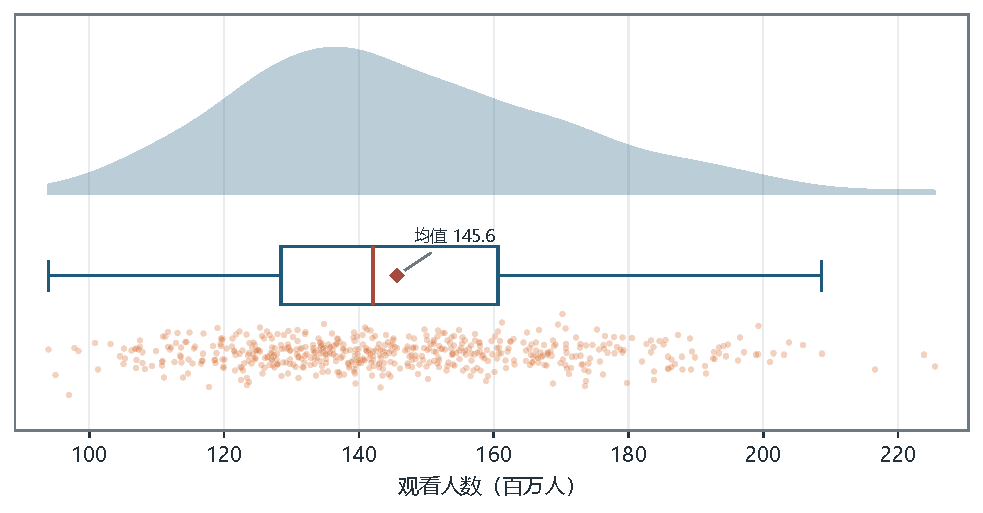
\includegraphics[width=0.72\textwidth,height=0.22\textheight,keepaspectratio]{../figures/fig_q1_target_raincloud.pdf}
\caption{训练集观看人数分布与右尾特征}
\label{fig:q1-target-raincloud}
\end{figure}

平均 Elo、平均排名、平均球迷基础与观看人数的线性相关系数约为 $0.62$、$-0.61$ 和 $0.69$，赔率熵约为 $0.31$。平均 Elo 与平均排名高度反向，特征之间存在明显共线；同一实力区间内的观看人数仍较分散，单变量也不足以解释需求。候选模型因此包括均值基线、Elastic Net、ExtraTrees 和 CatBoost，用同一时间折比较线性正则化与非线性机制。

Elastic Net 的估计量为
\begin{equation}
\widehat\beta=\arg\min_\beta\left\{
\frac{1}{n}\sum_{j=1}^{n}(Y_j-X_j^\top\beta)^2+
\alpha\left[\rho\lVert\beta\rVert_1+
\frac{1-\rho}{2}\lVert\beta\rVert_2^2\right]\right\}.
\end{equation}
网格取 $\alpha\in\{10^{-3},10^{-2},10^{-1},1,10\}$、$\rho\in\{0.1,0.5,0.9\}$，最终选择 $\alpha=1.0,\rho=0.9$。ExtraTrees 固定 $600$ 棵树并比较叶节点下限与特征比例；CatBoost 最多训练 $3000$ 轮，在折内末 $20\%$ 时间段早停。

\subsection{时间外验证与模型选择}

表\ref{tab:q1-model-summary-short}显示，Elastic Net 的平均 MSE 为 $220.086$，低于 CatBoost 的 $234.209$ 和 ExtraTrees 的 $250.162$；相对均值基线 $581.203$，MSE 降低约 $62.1\%$。RMSE 与 MAE 给出同一排序，说明选模结果不依赖单一损失口径。五折逐折误差及其稳定性在第\ref{sec:sensitivity}节继续检验。

\begin{table}[htbp]
\centering
\caption{候选模型时间外误差汇总}
\label{tab:q1-model-summary-short}
\begin{tabular}{lrrr}
\toprule
模型 & 平均 MSE & 平均 RMSE & 平均 MAE \\
\midrule
Elastic Net & 220.086 & 14.812 & 11.828 \\
CatBoost & 234.209 & 15.267 & 12.184 \\
ExtraTrees & 250.162 & 15.778 & 12.734 \\
均值基线 & 581.203 & 24.099 & 19.333 \\
\bottomrule
\end{tabular}
\end{table}

复杂模型没有抵消小样本方差：CatBoost 与 ExtraTrees 的 MSE 分别高出 $15.967$ 和 $30.076$。因此按预先规定的规则选择 Elastic Net，在全部 $560$ 条训练样本上重拟合，并保留 $465$ 条时间外 OOF 预测用于区间和残差分析。

\subsection{诊断、解释与预测输出}

OOF 拟合见图\ref{fig:q1-prediction-fit}。整体 $R^2$ 约为 $0.620$、RMSE 约为 $14.84$ 百万人；真实值超过约 $190$ 百万人后，预测更常落在 $45$ 度线下方，表明正则化模型对高关注赛事存在收缩性低估。残差均值为 $-0.00093$ 百万人，日期序列在 $2019$--$2024$ 年间围绕零线波动，没有持续同向漂移；Q--Q 尾部的轻微偏离说明经验区间比正态近似更合适。

\begin{figure}[htbp]
\centering
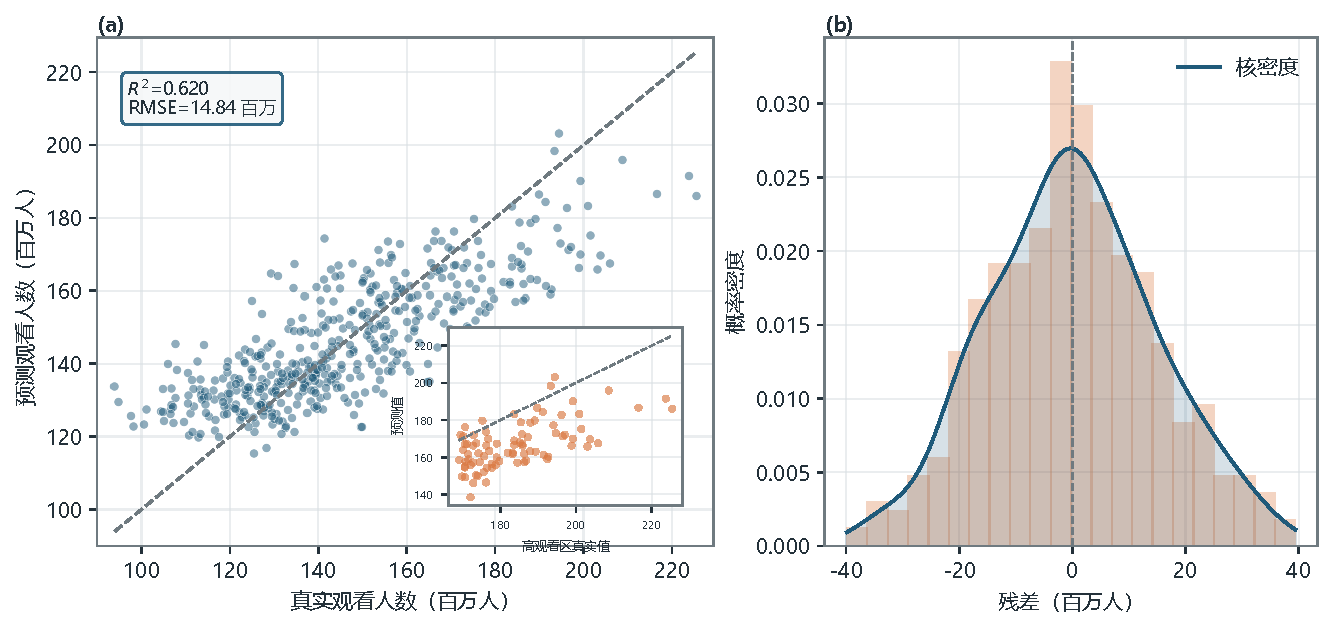
\includegraphics[width=0.80\textwidth,height=0.48\textheight,keepaspectratio]{../figures/fig_q1_prediction_fit.pdf}
\caption{最终模型 OOF 预测拟合与残差分布}
\label{fig:q1-prediction-fit}
\end{figure}

OOF 残差的 $5\%$ 与 $95\%$ 分位数分别为 $-22.7075$ 和 $25.1737$ 百万人。对点预测 $\widehat Y(x)$，本文使用
\begin{equation}
PI_{0.90}(x)=\left[\max\{0,\widehat Y(x)-22.7075\},\ \widehat Y(x)+25.1737\right]
\end{equation}
描述历史时间外误差；它不是严格的条件置信区间。

图\ref{fig:q1-shap-summary}给出后 $20\%$ 验证窗口的置换重要性和单样本影响。打乱平均球迷基础后 MSE 增加 $238.032$，高于世界杯标记 $32.597$、球迷基础--世界杯交互 $26.379$ 和实力--赔率熵交互 $24.145$。主要信号集中在少数连续特征及预先指定交互，解释了线性正则化为何优于当前非线性候选；这些数值只表示预测贡献，不表示因果效应。

\begin{figure}[htbp]
\centering
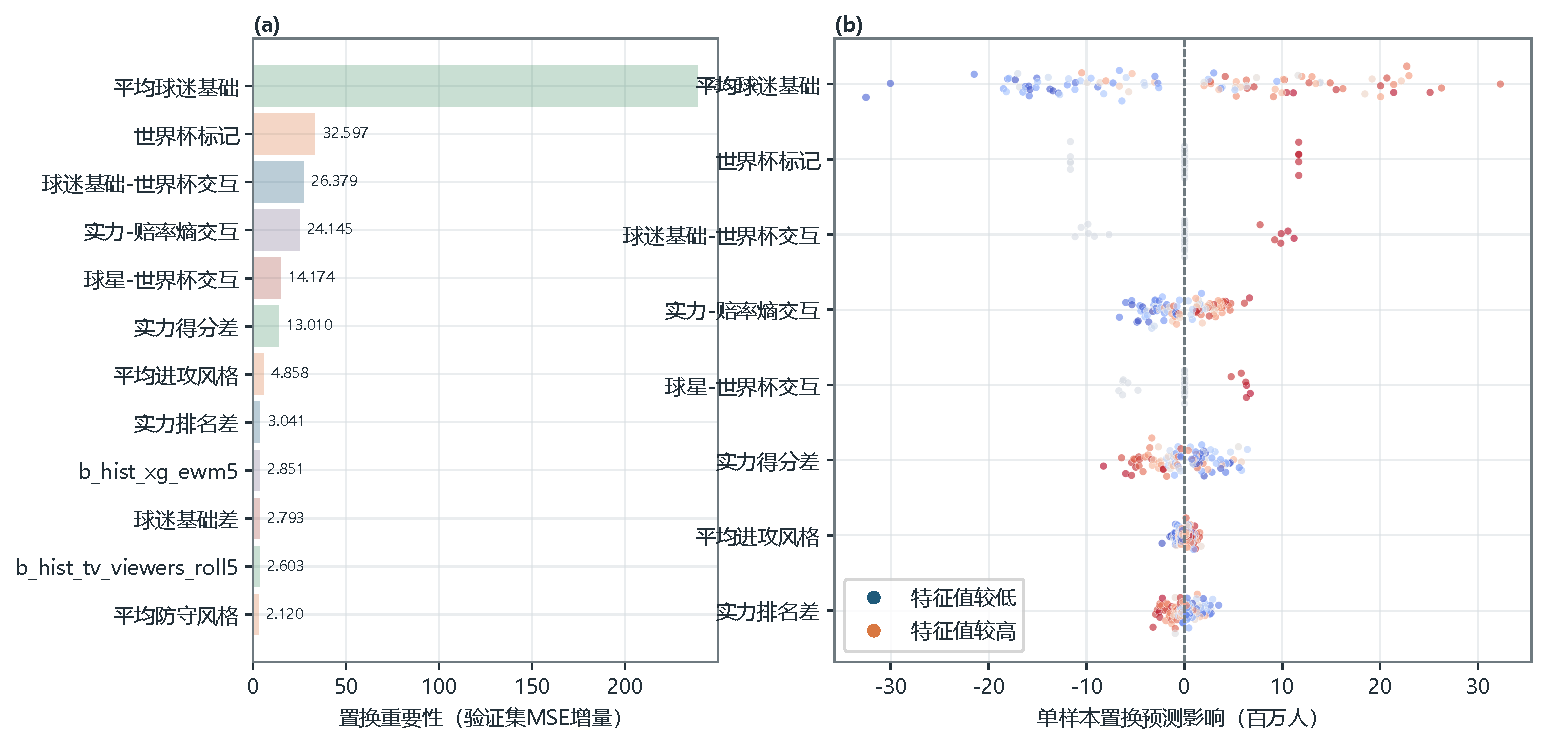
\includegraphics[width=0.82\textwidth,height=0.30\textheight,keepaspectratio]{../figures/fig_q1_shap_summary.pdf}
\caption{Elastic Net 置换重要性与单样本预测影响}
\label{fig:q1-shap-summary}
\end{figure}

最终模型对 $140$ 条测试记录的预测范围为 $115.783$--$188.216$ 百万人，均值 $145.331$ 百万人，均为有限正值。$72$ 场模拟小组赛的预测范围为 $144154622$--$205695590$ 人，均值 $170321280$ 人；两份结果保持模板主键、行数和单位。问题二只接收这 $72$ 场赛前点预测，不读取测试标签或赛后字段。

\section{问题二：场馆与开球时段协同优化}

\subsection{三维指派与候选域}

设比赛、场馆和参考时段集合为 $\mathcal I,\mathcal V,\mathcal S$。仅当场馆安保能力满足比赛需求时保留候选
\begin{equation}
\Omega=\{(i,v,s):L_v^{sec}\ge L_i^{req}\},
\end{equation}
并建立 $x_{ivs}\in\{0,1\}$；$y_v$ 表示场馆是否启用。当前数据形成 $85680$ 个三维布尔变量。场馆和时段同时决定当地日期、票务、转播、旅行与风险，因此不把问题拆成两个相互独立的贪心步骤。

比赛 $i$ 在场馆 $v$ 的预计上座为 $N_{iv}=\min(N_i^{pre},K_v)$。票务、转播和成本原值为
\begin{align}
T^0(x)&=\sum_{(i,v,s)\in\Omega}x_{ivs}P_{r(i)}^0N_{iv},\\
B^0(x)&=\sum_{(i,v,s)\in\Omega}x_{ivs}V_i^{pre}u_{r(i)}g_s^{prime}w_{r(i)}^{sponsor},\\
C^0(x,y)&=\sum_v10^6c_v^{setup}y_v+
\sum_{(i,v,s)\in\Omega}x_{ivs}\left(10^6c_v^{op}+10^5L_i^{req}c_v^{sec}\right).
\end{align}
费用统一换算为美元，场馆启用费只计一次。附件中所有场馆的最小承办数均为 $2$，故每个可行方案必启用全部 $16$ 个场馆，启用费在本数据中是共同常数。

\subsection{旅行、风险与公平指标}

旅行严格使用题面特殊口径。距离、旅行时间和时区差先在全部合法球队--轮次--候选场馆组合上分别 Min--Max，再按 $0.5,0.3,0.2$ 合成。第一轮从球队代表地出发；第二、三轮对球队 $t$ 和本轮场馆 $v$，以前一轮全部安保合格场馆为起点：
\begin{equation}
\bar q_{trv}=\frac{1}{|\mathcal V_{t,r-1}^{qual}|}
\sum_{u\in\mathcal V_{t,r-1}^{qual}}q_{uv},\qquad
q\in\{distance,time,timezone\}.
\end{equation}
每场取双方平均并对 $72$ 场求均值得到 $D$，不能替换成上一轮实际所选场馆的路径。

单场执行风险为
\begin{equation}
r_{iv}=0.5c_v^{climate}+0.3\frac{N_{iv}}{K_v}+0.2\frac{L_i^{req}}{L_v^{sec}},
\end{equation}
整套赛程取均值 $R$。悬念 $U$ 为 $72$ 场竞技悬念指数均值，吸引力 $H$ 为吸引力指数除以 $100$ 后的均值。若球队 $t$ 的黄金时段和大容量场馆次数分别为 $n_t^{prime},n_t^{large}$，公平惩罚为
\begin{equation}
F=\frac12\frac{\max_t n_t^{prime}-\min_t n_t^{prime}}3+
\frac12\frac{\max_t n_t^{large}-\min_t n_t^{large}}3.
\end{equation}
黄金时段取 $80$ 个候选时段中得分最高的 $20$ 个，大容量场馆取 $16$ 个场馆中容量最高的 $4$ 个；阈值并列未跨越名额切点。

\subsection{确定性的全部候选组合 Min--Max}

旧实现用六个限时辅助排程的对偶最好界作 $T,B,C$ 端点，等价表达式会改变搜索路径和端点，因而不适合作为可复现的评价尺度。本文改为直接枚举全部合法三元候选。对 $k\in\{T,B,C\}$，逐场在 $\Omega_i$ 中取候选最小和最大后汇总：
\begin{equation}
k_{min}=\sum_{i\in\mathcal I}\min_{(v,s)\in\Omega_i}k_i(v,s),\qquad
k_{max}=\sum_{i\in\mathcal I}\max_{(v,s)\in\Omega_i}k_i(v,s),
\end{equation}
其中 $C$ 的两端同时加入全部必启用场馆的一次性成本。任何满足联合约束的赛程都是该候选笛卡尔域的子集，故其指标必落在包络内；该计算不调用求解器、没有时间限制和随机性。得到
\begin{align}
T^0&\in[281888385,285910470],\\
B^0&\in[150900200.787,367190488.581],\\
C^0&\in[47730000,63910000].
\end{align}
三项用 $(k-k_{min})/(k_{max}-k_{min})$ 归一化；若端点相等则按题意置零。$U,H,D,F,R$ 已按上述定义位于 $[0,1]$。最终目标为
\begin{equation}
\max Z_2=0.25T+0.25B+0.15U+0.10H-0.08C-0.07D-0.06F-0.04R.
\end{equation}

\subsection{硬约束与求解设置}

模型逐项施加：每场恰好一次指派；同一场馆同一 UTC 时刻至多一场；球队按三轮顺序参赛且相邻轮至少休息 $60$ 小时；场馆当地日负荷和总负荷满足附件上下限；不建立安保不合格候选；同一时段比赛数不超过转播容量；第三轮高安保比赛逐参考日不超过动态容量；任意球队黄金时段次数极差不超过 $2$。核心形式包括
\begin{align}
\sum_{v,s}x_{ivs}&=1,&
\sum_i x_{ivs}&\le1,\\
\tau_{t,r+1}-\tau_{tr}&\ge60,&
\max_t n_t^{prime}-\min_t n_t^{prime}&\le2.
\end{align}
场馆日容量按所选 UTC 时刻转换到场馆 IANA 时区后的当地日期计算，动态资源容量则按附件参考日计算，两类日期不混用。

所有浮点目标系数乘 $10^6$ 转为整数。CP-SAT 固定单线程和随机种子 $20260813$，最长运行 $1800$ 秒，相对间隙阈值 $0.5\%$；先在宽轮次窗口内求可行提示，再在完整 $80$ 时段域求主目标。Python 3.11 的两次独立进程分别用时约 $173$ 与 $177$ 秒，Python 3.12 的干净环境复现用时约 $580$ 秒；三次均达到相同停止准则并生成逐字节相同的正式 CSV。

\subsection{结果与可执行性}

主方案原值为 $T^0=285581790$、$B^0=323423207.006$、$C^0=53075000$ 美元；八项标准化指标为
\begin{equation}
\begin{aligned}
(T,B,U,H)&=(0.918281,0.797646,0.461436,0.639699),\\
(C,D,F,R)&=(0.330346,0.201797,0.333333,0.416678).
\end{aligned}
\end{equation}
从而 $Z_2=0.484946$，高于同约束可行基线 $0.350742$。缩放目标的可行值为 $17811471$、最好界为 $17883841$，相对证书间隙约 $0.406\%$；因此 `OPTIMAL` 只按预设 $0.5\%$ 停止口径解释，不声称零间隙精确最优。

\begin{figure}[htbp]
\centering
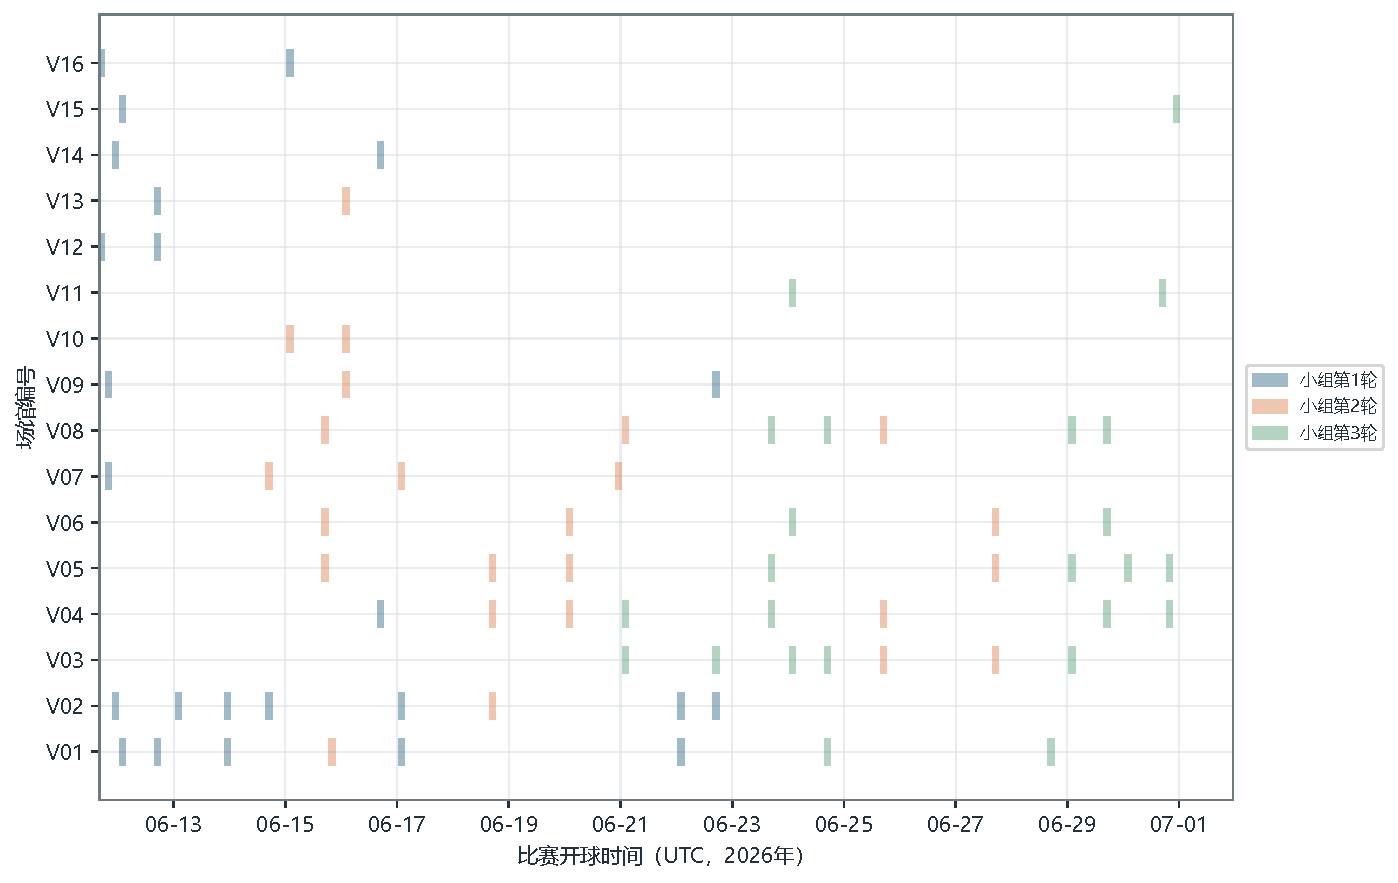
\includegraphics[width=0.88\textwidth,height=0.66\textheight,keepaspectratio]{../figures/fig_q2_schedule_gantt.pdf}
\caption{问题二最终 72 场 UTC 排程}
\label{fig:q2-schedule-gantt}
\end{figure}

\begin{table}[H]
\centering
\caption{问题二关键约束复算与裕度}
\label{tab:q2-constraint-audit}
\small
\begin{tabular}{lrrrrc}
\toprule
约束族 & 实际值 & 界值 & 单位 & 最小裕度 & 状态 \\
\midrule
最小轮间休息 & 63.000 & 60.000 & 小时 & 5.0\% & 通过 \\
场馆承办下界 & 0.000 & 0.000 & 剩余场 & 0.0\% & 通过 \\
场馆承办上界 & 0.000 & 0.000 & 剩余场 & 0.0\% & 通过 \\
场馆单日本地容量 & 1.000 & 1.000 & 最大利用率 & 0.0\% & 通过 \\
场馆安保等级 & 0.000 & 0.000 & 等级余量 & 0.0\% & 通过 \\
时段转播容量 & 0.000 & 0.000 & 剩余场 & 0.0\% & 通过 \\
第三轮高安保日容量 & 0.000 & 0.000 & 比例余量 & 0.0\% & 通过 \\
黄金时段公平极差 & 1.000 & 2.000 & 场 & 50.0\% & 通过 \\
\bottomrule
\end{tabular}
\vspace{2pt}
\noindent\begin{minipage}{0.96\textwidth}\footnotesize 注：裕度为按各约束自身上限归一化后的最小剩余比例；零表示约束在最紧样本上取等。\end{minipage}
\end{table}


独立从正式 CSV 复算：$72$ 个比赛编号完整且唯一，场馆--UTC 冲突为 $0$，最小轮间休息为 $63$ 小时；$16$ 个场馆各承办 $2$--$8$ 场，场馆当地日、安保、时段转播和第三轮高安保容量均无违反。黄金时段次数极差为 $1$，大容量场馆次数极差为 $1$。逐场票务、转播、旅行和风险字段与附件公式的最大数值误差低于 $10^{-8}$，总目标只写在 CSV 第一条记录。

\section{问题三：共同截面下的第三轮动态资源优化}

\subsection{信息边界与固定赛程}

问题三只处理问题二的 $24$ 场第三轮比赛。比赛编号、双方球队、场馆与开球时段全部锁定，决策仅包括转播优先级 $b_i$、安保等级 $q_i$、交通保障等级 $l_i$ 和票价调整比例 $\delta_i$。前两轮 $48$ 场反馈先汇总成唯一快照，再一次性模拟全部第三轮；任一第三轮模拟结果都不更新其他第三轮比赛参数。因此本问不是按日或按场滚动更新，而是附录图\ref{fig:flow-q3}所示的“共同截面--联合模拟--静动态并行求解--同界复评”。

\subsection{球队状态、进球均值与联合晋级模拟}

球队 $t$ 的前两轮场数、积分和红牌数记为 $G_t,P_t,RC_t$，累计预期进球与累计预期失球记为 $xGF_t,xGA_t$。严格采用题定状态式与伤病截断：
\begin{align}
S_t={}&0.45\frac{P_t}{3G_t}+0.35\left[0.5+0.5\tanh\!\left(\frac{(xGF_t-xGA_t)/G_t}{1.25}\right)\right]
+0.20\exp\!\left(-0.55\frac{RC_t}{G_t}\right),\\
h_t={}&\operatorname{clip}\!\left(\operatorname{mean}_{m\in\mathcal M_t^{1:2}}h_m,0,3\right).
\end{align}
对第三轮比赛 $i=(a,b)$，令
\begin{equation}
\Delta_i=0.32(S_a-S_b)-0.055(h_a-h_b),
\end{equation}
并在基础进球均值上更新
\begin{align}
\lambda_{i,a}&=\operatorname{clip}\!\left(\lambda^0_{i,a}e^{\Delta_i-0.04h_a},0.15,4.50\right),\\
\lambda_{i,b}&=\operatorname{clip}\!\left(\lambda^0_{i,b}e^{-\Delta_i-0.04h_b},0.15,4.50\right).
\end{align}

固定 PCG64 种子后，同时生成 $20000\times24$ 个独立泊松比分。每个样本先在 $12$ 个小组内依次按积分、净胜球、总进球排序，再把 $12$ 个第三名统一比较并选取最好 $8$ 队。完全同分块若跨越晋级线，就按该块可用名额质量等比例分配。因此每次模拟的晋级质量恒等于 $12\times2+8=32$，球队概率满足
\begin{equation}
p_t=\frac{1}{20000}\sum_{m=1}^{20000}w_{tm}^{\mathrm{adv}},qquad
\sum_{t=1}^{48}p_t=32.
\end{equation}
比赛晋级重要性为
\begin{equation}
Q_i=\frac{4p_a(1-p_a)+4p_b(1-p_b)}{2}.
\end{equation}
同一批样本还按本场平局、A 队胜、B 队胜三个条件计算条件晋级概率，用于后续默契风险，而没有再生成另一套不一致的随机样本。

基准种子下 $48$ 队概率位于 $[0.0023,1]$，数值和为 $32.000000$；更新进球均值位于 $[0.4752,3.0146]$。五个固定种子下单队概率标准差最大为 $0.00469$，主要概率位移见图\ref{fig:q3-advancement-shift}。

\begin{figure}[htbp]
    \centering
    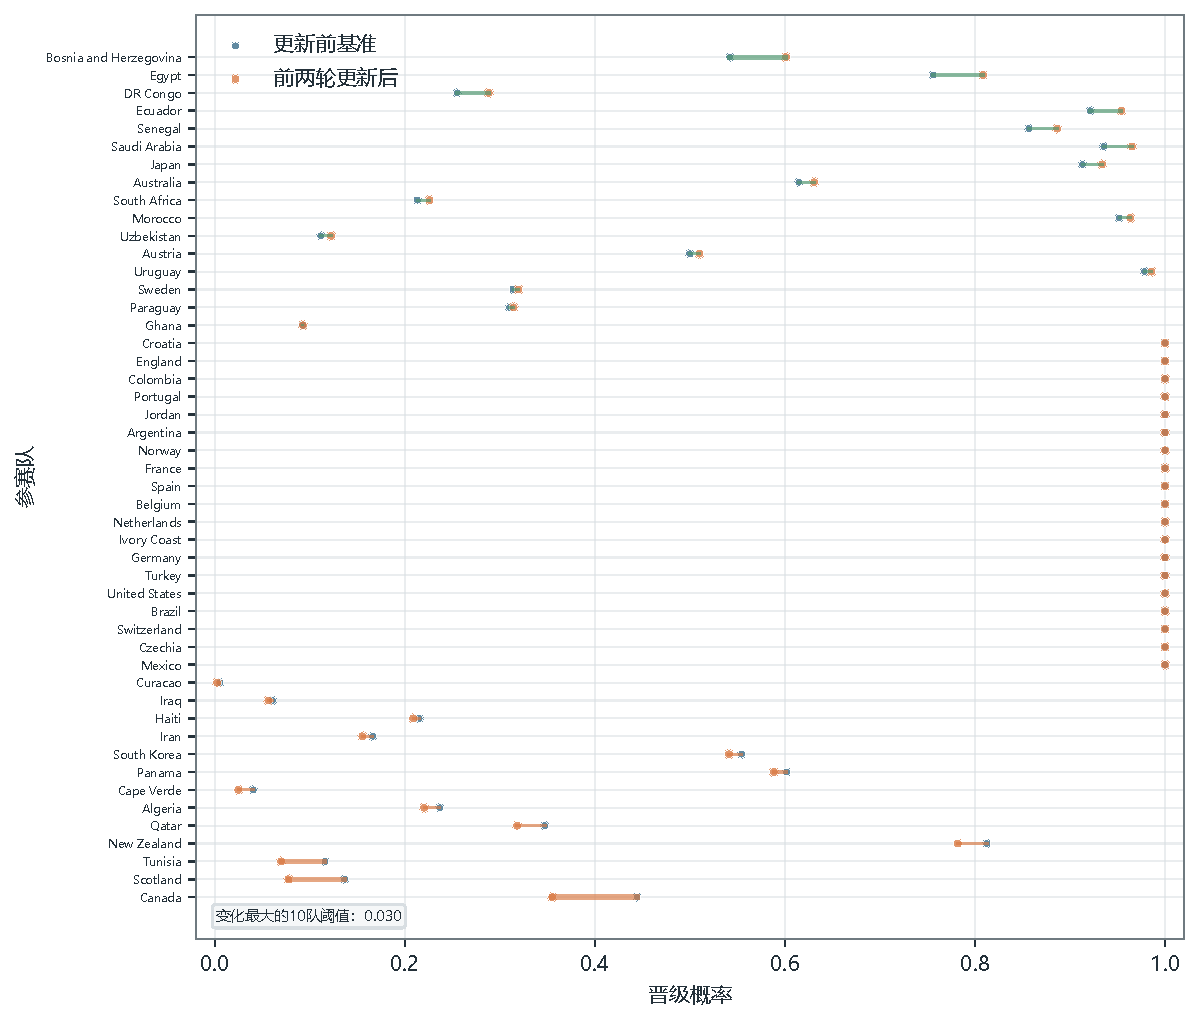
\includegraphics[width=0.82\textwidth,height=0.64\textheight,keepaspectratio]{../figures/fig_q3_advancement_shift.pdf}
    \caption{第三轮开始前的晋级概率更新}
    \label{fig:q3-advancement-shift}
\end{figure}

\subsection{反馈、需求与风险注册表}

对球队 $t$ 的每场前两轮比赛，先把实际/赛前预计现场观众比和转播观众比分别截断到 $[0.60,1.50]$，再取两场均值并截断到 $[0.75,1.25]$，得到 $r_t^N,r_t^V$。比赛层反馈取双方几何平均：
\begin{equation}
f_i^N=\sqrt{r_a^Nr_b^N},\qquad f_i^V=\sqrt{r_a^Vr_b^V}.
\end{equation}
令 $S_i=(S_a+S_b)/2$、$H_i=(h_a+h_b)/6$，以及
\begin{equation}
F_i=\operatorname{clip}\!\left(\frac{0.5f_i^N+0.5f_i^V-0.75}{0.50},0,1\right),
\end{equation}
则吸引力、资源配置前现场需求与转播需求依题定公式更新为
\begin{align}
A_i={}&\operatorname{clip}\!\left(0.50A_i^0+0.25Q_i+0.12F_i+0.08S_i+0.05(1-H_i),0,1\right),\\
\widetilde N_i={}&N_i^{pre}f_i^N(0.88+0.27Q_i)(0.94+0.12S_i)(1-0.10H_i),\\
\widetilde V_i={}&V_i^{pre}f_i^V(0.87+0.30Q_i)(0.90+0.20A_i)(1-0.06H_i).
\end{align}

从资源表读取交通需求倍率 $m_{l_i}^N$、转播需求倍率 $m_{b_i}^V$、安保剩余风险倍率 $m_{q_i}^R$ 和三类成本。附件给出的第三轮价格弹性为 $\varepsilon=-0.75$，票务价值在合法价格域内随 $\delta$ 单调增加，故可先解析消去连续变量：
\begin{equation}
\delta_i^*=\min\left\{\delta_{d(i)}^+,\ 0.88^{1/\varepsilon}-1\right\},
\end{equation}
该值同时满足 $-\delta_{d(i)}^-\le\delta_i^*\le\delta_{d(i)}^+$。最终现场人数、票务价值、转播人数和转播价值为
\begin{align}
N_i(\delta_i^*)&=\min\{K_i,\widetilde N_i m_{l_i}^N(1+\delta_i^*)^{\varepsilon}\},
&TV_i&=P_i^0(1+\delta_i^*)N_i(\delta_i^*),\\
V_i&=\widetilde V_i m_{b_i}^V,
&BV_i&=u_iV_i.
\end{align}
程序逐动作验证 $N_i(\delta_i^*)\ge0.88N_i(0)$，没有把需求底线留到导出后修补。

无激励风险、默契风险、动态安保需求与综合风险分别为
\begin{align}
R_i^{stake}&=0.5(2p_a-1)^2+0.5(2p_b-1)^2,\\
D_i&=\min(p_a^D,p_b^D),\quad
G_i=0.5[p_a^W-p_a^D]_++0.5[p_b^W-p_b^D]_+,\\
R_i^{col}&=\operatorname{clip}\!\left(D_i[1-\operatorname{clip}(G_i,0,1)](1-0.35R_i^{stake}),0,1\right),\\
d_i&=\operatorname{clip}\!\left(0.45d_i^0+0.25O_i+0.15A_i+0.15\frac{R_i^{stake}+R_i^{col}}2,0,1\right),\\
R_i&=0.40R_i^{stake}+0.40R_i^{col}+0.20d_im_{q_i}^R,qquad
O_i=\operatorname{clip}(\widetilde N_i/K_i,0,1).
\end{align}

\subsection{静态基线、动态动作与日级约束}

每场枚举 $b_i\in\{1,2,3\}$、$q_i\in\{L_i^{req},\ldots,L_{v(i)}^{sec}\}$、$l_i\in\{1,2,3\}$，票价取上式解析最优值。资源成本为 $C_i=c_{b_i}+c_{q_i}+c_{l_i}$。在全部更新动作上一次计算 $TV,BV,A,C,R$ 的共同 Min--Max 边界，目标为
\begin{equation}
\max Z_3=\sum_{i\in I_3}\left(0.35TV_i'+0.35BV_i'+0.10A_i'-0.10C_i'-0.10R_i'\right).
\end{equation}
对每个实际出现的参考日 $d$，同时施加
\begin{align}
\sum_{i\in I_d}\mathbf 1(b_i=3)&\le H_d^B,&
\sum_{i\in I_d}\mathbf 1(q_i\ge3)&\le H_d^S,\\
\sum_{i\in I_d}\mathbf 1(l_i=3)&\le H_d^L,&
\sum_{i\in I_d}C_i&\le B_d.
\end{align}

静态方案不是默认档位：它先用赛前需求、赛前吸引力及题定赛前风险，在完全相同的动作集合和日约束下独立优化；前两轮结束后四项决策锁定，只把该动作放入更新环境重评。动态方案则在更新环境中重新优化。两者最终均使用更新动作域的同一组边界计分，故 $Z_3^{static}$ 与 $Z_3^{dynamic}$ 可直接比较；模型中不存在“变更惩罚”或另一套分资源预算。

\begin{table}[H]
\centering
\caption{问题三逐日动态资源使用与容量}
\label{tab:q3-resource-budget}
\small
\resizebox{\textwidth}{!}{%
\begin{tabular}{lrrrrrrrrc}
\toprule
日期 & 高转播 & 转播上限 & 高安保 & 安保上限 & 强化交通 & 交通上限 & 预算使用 & 预算上限 & 状态 \\
\midrule
2026-06-20 & 2 & 4 & 1 & 3 & 2 & 4 & 35.0 & 120 & 通过 \\
2026-06-22 & 1 & 3 & 0 & 3 & 0 & 3 & 13.0 & 100 & 通过 \\
2026-06-23 & 3 & 3 & 3 & 3 & 3 & 3 & 86.0 & 100 & 通过 \\
2026-06-24 & 3 & 3 & 1 & 2 & 3 & 3 & 51.0 & 100 & 通过 \\
2026-06-28 & 4 & 4 & 3 & 3 & 4 & 4 & 77.0 & 120 & 通过 \\
2026-06-29 & 3 & 3 & 2 & 2 & 2 & 3 & 54.0 & 100 & 通过 \\
2026-06-30 & 3 & 3 & 2 & 2 & 3 & 3 & 59.0 & 100 & 通过 \\
\bottomrule
\end{tabular}
}
\end{table}


新问题二赛程使第三轮分布在 $7$ 个参考日。表\ref{tab:q3-resource-budget}逐日给出三级转播、三级及以上安保、三级交通和总预算使用量，所有不等式均通过；安保档位还逐场满足最低需求且不超过固定场馆能力。

\subsection{结果、同界增益与随机稳定性}

\begin{table}[H]
\centering
\caption{问题三静态策略与动态重优化同界比较}
\label{tab:q3-static-dynamic}
\small
\begin{tabular}{lrrrr}
\toprule
指标 & 静态策略重评 & 动态重优化 & 偏好方向改善 & 单位 \\
\midrule
票务价值 TV & 113.715 & 113.385 & -0.330 & 百万美元 \\
转播价值 BV & 168.309 & 168.368 & 0.059 & 百万美元 \\
吸引力 A & 0.512 & 0.512 & 0.000 & 无量纲 \\
资源成本 C & 396.000 & 375.000 & 21.000 & 成本指数 \\
风险 R & 0.465 & 0.469 & -0.004 & 无量纲 \\
综合目标 Z3 & 6.572230 & 6.637484 & 0.065254 & 无量纲 \\
\bottomrule
\end{tabular}
\vspace{2pt}
\noindent\begin{minipage}{0.96\textwidth}\footnotesize 注：正的偏好方向改善表示动态方案更优；成本与风险按越低越优转换。\end{minipage}
\end{table}


静态锁定方案在更新环境中的同界得分为 $6.572230$，动态重优化得分为 $6.637484$，净增量为 $0.065254$；$24$ 场中 $8$ 场改变至少一个资源决策。表\ref{tab:q3-static-dynamic}显示，动态方案票务价值减少 $0.330$ 百万美元、转播价值增加 $0.059$ 百万美元、资源成本指数减少 $21$，风险均值增加约 $0.004$。因此增益来自题定五指标的全局权衡，而不是不存在的改动成本。

\begin{figure}[htbp]
    \centering
    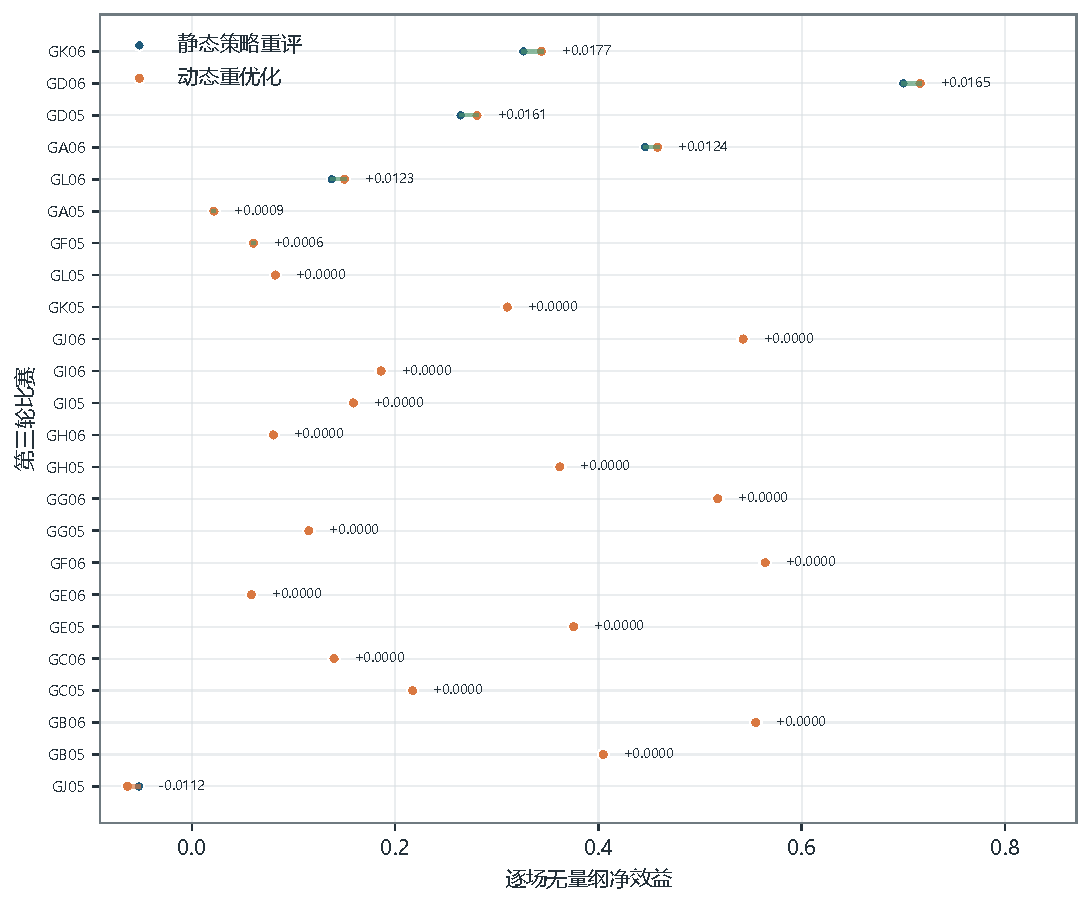
\includegraphics[width=0.84\textwidth,height=0.66\textheight,keepaspectratio]{../figures/fig_q3_dynamic_value_dumbbell.pdf}
    \caption{静态锁定方案与动态重优化的逐场同界净价值}
    \label{fig:q3-dynamic-value-dumbbell}
\end{figure}

五个种子均重新执行 $20000\times24$ 联合模拟、条件概率计算、环境更新和完整动态 CP-SAT。五次动态求解均为 `OPTIMAL`，增益位于 $[0.065123,0.065434]$，相对基准种子的 $24$ 场动态资源决策均无变化。这说明本次配置差异不是由单个随机种子的抽样波动驱动。

\section{问题四：真实世界杯赛程的双层同口径评价}

\subsection{比较边界与数据来源}

本问选取 $2022$ 年卡塔尔世界杯小组赛作为现实参照。机器读取源为工作区保存的 OpenFootball 结构化 JSON，FIFA 官方赛程与比分页面用于逐场核验；场馆容量取 FIFA 赛后统计，坐标按 FIFA 场馆地址核对\upcite{openfootball_2022,fifa_qatar_schedule,fifa_qatar_at_glance}。实际赛程的 $48$ 场记录逐行保存球队、轮次、场馆、当地开球时间、UTC 时间和机器来源链接，不再把“采集源”与“官方核验源”写成同一字段。附件中的空白模板仅规定提交字段，不被当作观测数据；UTC 时间根据当地时间和 IANA 时区重新计算。

实际赛程与问题二的 $72$ 场方案在球队规模、比赛数量和场馆集合上并不相同，直接比较总收益会把规模效应误当作安排优劣。为此，我们设置双层评价：第一层由两套赛程共同调用一个结构函数，比较休息、跨时区、实际场馆旅行、场馆日负荷、容量匹配、黄金覆盖和预计观众；第二层先将现实比赛与场馆整体映射到问题二候选域，再复算问题二八指标。

流程的关键不是寻找一个绝对“冠军方案”，而是保持比较口径对称。结构层的每一项均有明确物理单位和规模分母；代理层的现实比赛与场馆分别整体映射到问题二的比赛和安保合格候选场馆，随后使用问题二相同的距离、时间、时区边界与权重。现实数据无法直接识别的商业、安保和题内吸引力统一标记为代理量，并与可观测结构分开解释。

\subsection{结构层的共同计算函数}

设球队 $t$ 的相邻两场比赛为 $j-1,j$，UTC 开球时刻为 $u_{tj}$，场馆坐标为 $(\phi_{tj},\lambda_{tj})$，场馆 UTC 偏移为 $z_{tj}$。休息、场馆旅行和跨时区指示分别定义为
\begin{equation}
r_{tj}=u_{tj}-u_{t,j-1},\qquad
d_{tj}=\operatorname{Haversine}\!\left((\phi_{t,j-1},\lambda_{t,j-1}),(\phi_{tj},\lambda_{tj})\right),
\end{equation}
\begin{equation}
c_{tj}=\mathbb I\!\left(z_{tj}\ne z_{t,j-1}\right).
\end{equation}
休息报告全部球队相邻轮间隔的最小值和平均值；旅行距离、换馆率和跨时区率均以球队转场次数为分母。场馆日利用率以“发生比赛的场馆日数”除以“启用场馆数乘比赛日期数”，场馆日峰值取单一场馆单日最大比赛数。容量匹配率为逐场 $\min(N_i/K_i,1)$ 的均值，黄金覆盖率和场均预计观众均以比赛场次为分母。两套赛程只传入字段名不同，计算公式和聚合方式完全相同。

\begin{table}[H]
\centering
\caption{两套赛程的可观测结构与规模强度比较}
\label{tab:q4-structural-comparison}
\small
\resizebox{\textwidth}{!}{%
\begin{tabular}{lllrrl}
\toprule
指标 & 定义与分母 & 单位 & 2022实际 & 2026优化 & 偏好方向 \\
\midrule
最小休息 & 球队相邻比赛 UTC 间隔的最小值 & 小时 & 87.0000 & 63.0000 & 越高越优 \\
平均休息 & 球队相邻比赛 UTC 间隔的平均值 & 小时 & 97.8125 & 139.8125 & 越高越优 \\
跨时区次数 & 相邻比赛场馆 UTC 偏移发生变化的次数 & 次 & 0 & 78 & 越低越优 \\
跨时区率 & 跨时区次数除以球队转场次数 & 比例 & 0.0000 & 81.2500 & 越低越优 \\
场馆旅行 & 相邻比赛实际场馆大圆距离的平均值 & 公里/次 & 18.9868 & 2019.1075 & 越低越优 \\
换馆率 & 相邻轮更换场馆的球队转场比例 & 比例 & 78.1250 & 94.7917 & 越低越优 \\
场馆日利用率 & 发生比赛的场馆日占可用场馆日比例 & 比例 & 45.1923 & 25.0000 & 越高越优 \\
场馆日峰值 & 单一场馆单日承办场次最大值 & 场/场馆日 & 2 & 1 & 越低越优 \\
容量匹配 & 预计现场观众与场馆容量之比的场均值 & 比例 & 81.7689 & 61.7245 & 越高越优 \\
黄金覆盖 & 按赛事进度日和 UTC 钟点映射后落入前四分位时段的比例 & 比例 & 25.0000 & 62.5000 & 越高越优 \\
场均预计观众 & 预计现场观众总量除以比赛场次 & 人/场 & 41451.67 & 41704.92 & 越高越优 \\
\bottomrule
\end{tabular}
}
\vspace{2pt}
\noindent\begin{minipage}{0.96\textwidth}\footnotesize 注：休息、时区、场馆路径与场馆日由逐场赛程直接复算；黄金覆盖来自唯一时段映射，容量匹配和预计观众的需求端为题内赛前代理。实际赛程有64次球队转场，优化赛程有96次。\end{minipage}
\end{table}


结构层逐项比较见表\ref{tab:q4-structural-comparison}。实际赛程最小休息为 $87$ 小时，高于优化方案的 $63$ 小时；但优化方案平均休息达到 $139.8125$ 小时，高于实际赛程的 $97.8125$ 小时，说明优化方案的休息分布更不均匀。卡塔尔赛程位于同一时区，$64$ 次球队转场中没有跨时区；跨国优化赛程的 $96$ 次转场中有 $78$ 次跨时区，平均场馆旅行距离也由 $18.9868$ 公里升至 $2019.1075$ 公里。

场馆运营维度呈现另一组取舍。实际与优化方案的场馆日峰值分别为 $2$ 场和 $1$ 场；场馆日利用率分别为 $45.1923\%$ 和 $25.0000\%$。基于同一赛前需求代理，两者的平均容量匹配率分别为 $81.7689\%$ 和 $61.7245\%$，场均预计现场观众分别为 $41451.67$ 和 $41704.92$ 人。按后述唯一时段映射，优化方案的黄金时段覆盖率为 $62.5000\%$，高于实际赛程的 $25.0000\%$；该项属于时间映射指标，不能替代跨时区和长距离旅行负担。

为统一展示不同物理单位下的方向和相对幅度，图\ref{fig:q4-schedule-difference}先按两方案绝对值最大者归一每个结构指标，再把“优化更符合偏好”记为正值。原始小时、公里、场次与比例仍以表\ref{tab:q4-structural-comparison}为准。

\begin{figure}[htbp]
    \centering
    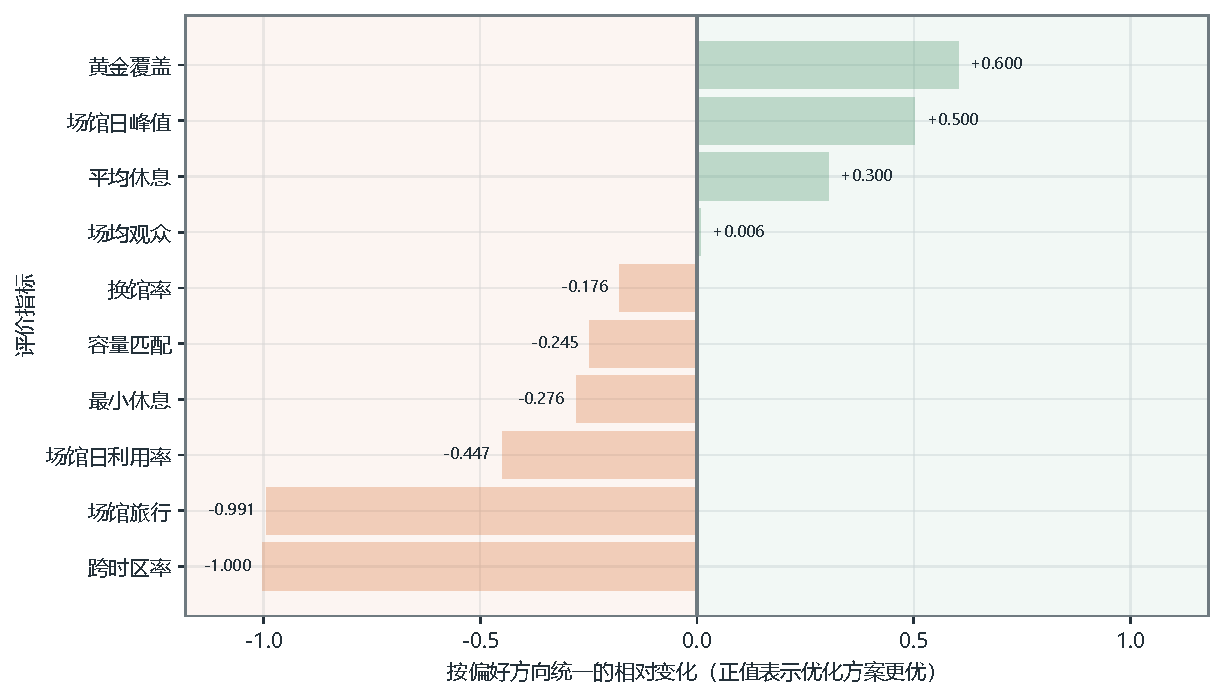
\includegraphics[width=0.85\textwidth,height=0.80\textheight,keepaspectratio]{../figures/fig_q4_schedule_difference.pdf}
    \caption{两套赛程的结构指标相对差异}
    \label{fig:q4-schedule-difference}
\end{figure}

\subsection{代理层的同构映射与强度化}

对受比赛数量影响的总量先做场均强度化。若方案 $s$ 有 $n_s$ 场比赛，则电视价值、品牌价值和成本分别写为
\begin{equation}
\bar T_s=\frac{T_s^0}{n_s},\qquad
\bar B_s=\frac{B_s^0}{n_s},\qquad
\bar C_s=\frac{C_s^0}{n_s}.
\end{equation}
旅行与风险使用逐场均值，$U,H$ 本身已是均值，公平性 $F$ 是每队三场资源次数极差的标准化结果。对 $T,B,C$，先将问题二候选上下界除以 $72$ 转为场均边界，再与基准实际、优化及第二近邻三个已报告场景的原始值取共同包络。两个方案随后共享这一组边界执行一次 Min--Max，既保留共同参照，又保证进入 $Z_4$ 的八项值严格属于 $[0,1]$。

实际赛程缺少与题目附件完全同构的商业和安保字段。为避免目标型特征和静默缺失填补，本文引入 $2022$ 年 $11$ 月 $12$ 日完整的世界杯赛前 Elo 快照\upcite{international_football_elo_2022}，覆盖全部 $32$ 支球队。比赛距离只使用双方 Elo 均值与差、由 Elo 构造的胜平负概率、不确定性和组内轮次，在题内 $72$ 场中寻找最近邻，再整体继承基础需求、吸引力与安保向量；预测观看人数不再参与邻居距离。实际场馆只依据有官方来源的容量，在满足该场安保等级的题内场馆中映射成本参数，不再声称使用逐场馆气候或公共交通数据。风险中的气候项固定为透明情景值 $0.12$。$U$ 不继承邻居，而由同一组三向赛前概率直接计算：
\begin{equation}
U_i=1-\max\{p_{ia},p_{iD},p_{ib}\}.
\end{equation}
黄金时段也复用问题二规则：先固定附件 $80$ 个候选时段中得分最高的 $20$ 个。为消除不同日期具有相同时钟距离时由行顺序决定结果的问题，先把现实赛程的 $13$ 个比赛日按赛事进度线性映射到模拟赛程的 $20$ 个候选日，再在对应日期内选择圆周 UTC 钟点距离最近的时段；若距离仍相同，则按时段编号稳定选择。由此每场现实比赛得到唯一、可复算的候选时段。

为保证两套赛程的旅行指标具有相同物理定义，现实赛程的每场比赛和场馆先整体映射到问题二索引，再调用问题二同一个旅行负担表；不把卡塔尔实际路径公里数除以全球最大距离后直接与问题二复合量混列：
\begin{equation}
D_i=\frac{1}{2}\sum_{t\in\{a_i,b_i\}}
\left(0.5\widetilde d_{tiv}+0.3\widetilde h_{tiv}+0.2\widetilde z_{tiv}\right).
\end{equation}
其中三项边界、第二三轮上一轮安保合格场馆集合与问题二完全一致。真实场馆路径仍在结构层以公里报告，不再进入这一复合量。

综合目标仅作为给定映射体系下的条件性分数：
\begin{equation}
Z_4=0.25T'+0.25B'+0.15U+0.10H-
\left(0.08C'+0.07D'+0.06F+0.04R\right).
\end{equation}

\subsection{代理指标结果与稳健性边界}

同构映射后，实际赛程的代理指标为 $T'=0.413433$、$B'=0.633928$、$U=0.441275$、$H=0.649119$、$C'=0.534340$、$D'=0.213022$、$F=0.666667$、$R=0.455654$；优化方案对应为 $0.918281$、$0.797646$、$0.461436$、$0.639699$、$0.382445$、$0.201797$、$0.333333$ 和 $0.416678$。八项值均位于 $[0,1]$，不再存在边界外推后由单一指标主导综合分的问题；各指标证据等级及单位列于附录表\ref{tab:q4-metric-definition}。

条件性代理层的共同尺度轮廓见附录图\ref{fig:q4-metric-radar}：优化方案在 $T,B,U,C,D,F,R$ 上更符合目标方向，实际赛程仅在 $H$ 上略高。成本、旅行、公平和风险在作图时只反转偏好方向，不再按两方案最大值二次缩放。由于这些指标的证据等级不同，雷达轮廓只能说明题内映射下的取舍，不能替代结构层的小时和公里结果。

基准最近邻代理下，实际赛程的 $Z_4$ 为 $0.277058$，优化赛程为 $0.480778$。逐一将八个权重的绝对值乘以 $0.9$ 和 $1.1$ 后重新归一，共形成 $16$ 个扰动情景：实际分位于 $[0.267908,0.285763]$，优化分位于 $[0.469560,0.491449]$，方向保持率为 $100\%$。将实际比赛与场馆代理整体换成第二近邻后，实际方案的 $Z_4$ 为 $0.226072$，优化方向仍保持。

修复后的代理方向在已检验权重和邻居替换下稳定，但证据边界仍不能省略：$48$ 场现实比赛映射到 $26$ 个题内比赛，单一比赛最多复用 $6$ 次；场馆成本代理只覆盖 $4$ 个题内场馆，其中一个被复用 $33$ 次。因此可以报告“当前题内映射下优化方案条件性总分较高”，却不能据此断言 FIFA 现实排程总体较差。抽签规则、转播合同、场馆可用性、当地治理、球队迁移策略和商业谈判等现实约束并未被附件完整观察；若用于现实决策，仍须补充真实合同、场馆运营和安保成本数据后重新校准代理层。

\section{结论、评价与适用边界}

\subsection{主要结论}

\begin{enumerate}
\setlength{\itemsep}{2pt}
\setlength{\parsep}{0pt}
  \item 在严格赛前信息边界和整窗标签屏蔽下，Elastic Net 的五折平均 MSE、RMSE 和 MAE 分别为 $220.0855$、$14.8121$ 和 $11.8276$，均优于另外三类候选。$72$ 场需求预测均值为 $170321280$ 人；高关注赛事的不确定性由 OOF 残差分位数单独给出。
  \item 三维 CP-SAT 联合决定 $72$ 场比赛的场馆与时段，得到 $Z_2=0.484946$。独立复算显示无硬约束违反，最小相邻轮休息为 $63$ 小时，场馆负荷为 $2$--$8$ 场；$0.41\%$ 的证书间隙满足预设停止准则，但不构成零间隙最优证明。
  \item 在第二轮结束的共同截面上，联合模拟保持每个样本的晋级名额质量为 $32$。动态方案仅调整 $8/24$ 场，目标由锁定静态方案的 $6.572230$ 提高到 $6.637484$；五种子完整重优化的增益为 $0.065123$--$0.065434$，离散决策一致。
  \item 实际赛程与优化方案存在结构取舍：实际赛程最小休息更长、跨时区和实际旅行更少，优化方案平均休息和黄金覆盖更高。共同边界下的代理综合分为 $0.277058$ 与 $0.480778$，权重和邻居扰动均保持方向；该结果只适用于题内映射，不能解释为 FIFA 现实排程的总体优劣。
\end{enumerate}

\subsection{可核验性}

四问按信息产生顺序连接：问题一只读开球前字段，问题二接收赛前需求，问题三在第二轮结束后更新状态，问题四才引入现实记录和代理。需求预测以“人”为单位进入排程；求解完成后，独立程序从正式 CSV 复算唯一指派、UTC 冲突、休息、容量、安保、日负荷与公平指标。求解器状态说明搜索程度，物理可行性由这些复算结果决定。

静态与动态方案共用动作域、更新环境、价格边界和归一化上下界，因此增益可以直接比较。现实评价则保留数据来源和代理标记：结构量按小时、公里和比例报告，缺失商业字段不伪装成观测。灵敏度分析进一步说明哪些扰动只改变数值，哪些可能改变离散动作，以及哪些结论仍受代理集中限制。

\subsection{局限与使用范围}

需求样本只有 $560$ 条，高观看尾部稀缺，Elastic Net 对极端赛事存在收缩性低估；特征重要性表示预测贡献，不是因果效应。排程模型受题定候选场馆、旅行口径和成本参数约束，未包含真实转播合同、临时管制、训练基地和维护窗口。动态模型采用泊松比分与离散资源档位，并固定第三轮共同截面；实际执行时，更新频率还必须服从通知提前量和资源调度周期。

问题四的商业价值、成本和安保字段来自代理，且映射存在复用集中。真实运营数据补齐前，$Z_4$ 只能描述条件性取舍，不能触发“替换现实排程”的决策。迁移到其他赛事时，可复用的是“需求预测--联合指派--滚动重评--独立审计”的结构；轮次规则、候选场馆、休息下限和资源预算必须按新场景重建。若真实约束无法进入模型或代理稳定性不足，应停止输出总体优劣，改为报告局部方案和待补数据。


% === 参考文献 ===
\bibliographystyle{gbt7714-numerical}
% === AI 工具使用声明（自动插入）===
\section*{AI 工具使用声明}
\addcontentsline{toc}{section}{AI 工具使用声明}
本参赛队在竞赛过程中使用了 AI 工具，主要用于论文技术审阅、题面--公式--代码一致性核查、代码调试、数值复算、LaTeX 排版与语言整理，详细使用情况见支撑材料。

\begingroup
\small
\bibliography{references}
\endgroup

% === 附录（格式规范规定页数不限）===
\clearpage
\appendix
\section{灵敏度分析与模型检验}

\subsection{预测模型的时间外检验}

问题一没有使用随机打乱的交叉验证，而是让每个验证窗口严格晚于训练窗口，并在特征重建前把该窗全部观看标签置空。五折扩窗检验的总体结果为 MSE $220.0855$、RMSE $14.8121$、MAE $11.8276$，OOF 残差均值为 $-0.001$ 百万人，说明预测误差在时间外样本上没有明显系统偏移。残差的 $5\%$ 和 $95\%$ 分位数分别为 $-22.7075$ 与 $25.1737$ 百万人，区间两侧大致均衡，但高观看场次仍有一定收缩性低估。因此，预测值适合进入排程模型做相对需求排序，极端场次则应结合经验残差区间保留容量冗余。

为了确认模型选择并非由单一指标偶然决定，我们同时比较 MSE、RMSE 与 MAE。Elastic Net 的三项误差均低于 CatBoost、ExtraTrees 和滚动均值基线，其中相对基线的 RMSE 由 $24.099$ 降至 $14.812$，降幅约 $38.5\%$；相对 CatBoost 的 RMSE 优势为 $0.455$ 百万人，且线性稀疏结构更容易审计赛前字段是否越界。模型选择因此同时满足精度、稳定性和可解释性，而不是只追求训练集上的最低误差。

问题一的另一项检验是把预测输出与后续决策变量解耦。排程优化只接收赛前点预测和经验误差边界，不把实际观看量或赛果重新写回特征表；问题三则在比赛结束后通过独立的状态更新模块改变概率和需求。前后两个时间截面的输入不同但接口清晰，避免了“用赛后事实证明赛前预测准确”的循环论证。

最终模型在五个连续外折上的误差列于表\ref{tab:q1-fold-stability}。训练窗逐步扩展时，RMSE 从 $15.5929$ 总体下降到 $13.2908$，第五折没有因时间距离更远而恶化；第二至第四折虽有波动，但全部低于 $15.5$ 百万人。五折 MSE 的最大值与最小值分别为 $243.1382$ 和 $176.6463$，说明总体均值 $220.0855$ 不是由单个异常折主导。

\begin{table}[htbp]
\centering
\caption{Elastic Net五个时间外折的误差稳定性}
\label{tab:q1-fold-stability}
\begin{tabular}{crrr}
\toprule
外折 & MSE & RMSE & MAE \\
\midrule
1 & 243.1382 & 15.5929 & 12.7572 \\
2 & 226.6187 & 15.0539 & 11.9290 \\
3 & 239.3400 & 15.4706 & 12.2031 \\
4 & 214.6845 & 14.6521 & 11.5100 \\
5 & 176.6463 & 13.2908 & 10.7386 \\
\bottomrule
\end{tabular}
\end{table}

分折结果还提供了部署期监测基准。若新增赛事窗口的 RMSE 超过当前最差折 $15.5929$ 很多，且误差集中在新的赛事类别或时区组合，应优先检查分布漂移和类别编码，而不是直接改变正则化参数；若残差均值显著偏离零，则说明模型出现系统高估或低估，需要重新校准截距或目标尺度。只有当这些诊断在连续窗口复现，才有依据触发完整重训。

验证窗目标历史采用统一口径：每一外折及最早外折的内部调参窗都先屏蔽整段观看标签，再重建目标滞后特征；较早比赛的进球、射门等其他已发生事实仍可滚动进入。该严格口径下 Elastic Net 的 MSE 为 $220.086$，四模型排序与最终 $140+72$ 条预测稳定，说明主结论不依赖验证窗内标签的递推可见性。

\subsection{排程目标权重敏感性}

问题二包含八个经同域归一化的目标分量，基准权重体现价值、观赏性、成本、旅行、公平和风险之间的折中。为检验固定方案对偏好变化的响应，我们在价值权重和风险惩罚权重的二维网格上重新评价已求得赛程；此处只改变评价权重，不重新求解整数规划，因此结果衡量的是“既定方案的评分敏感性”，而不是不同权重下的全局最优前沿。

固定方案在权重网格上的得分变化见图\ref{fig:q2-weight-sensitivity-contour}：取值从 $0.445463$ 变化到 $0.522504$，基准权重比 $(1,1)$ 处为 $0.484946$。价值权重上升时等高线整体向高分方向移动，惩罚权重增加则压低得分；曲面连续且没有局部突跳，说明归一化和符号方向设置一致。

\begin{figure}[htbp]
    \centering
    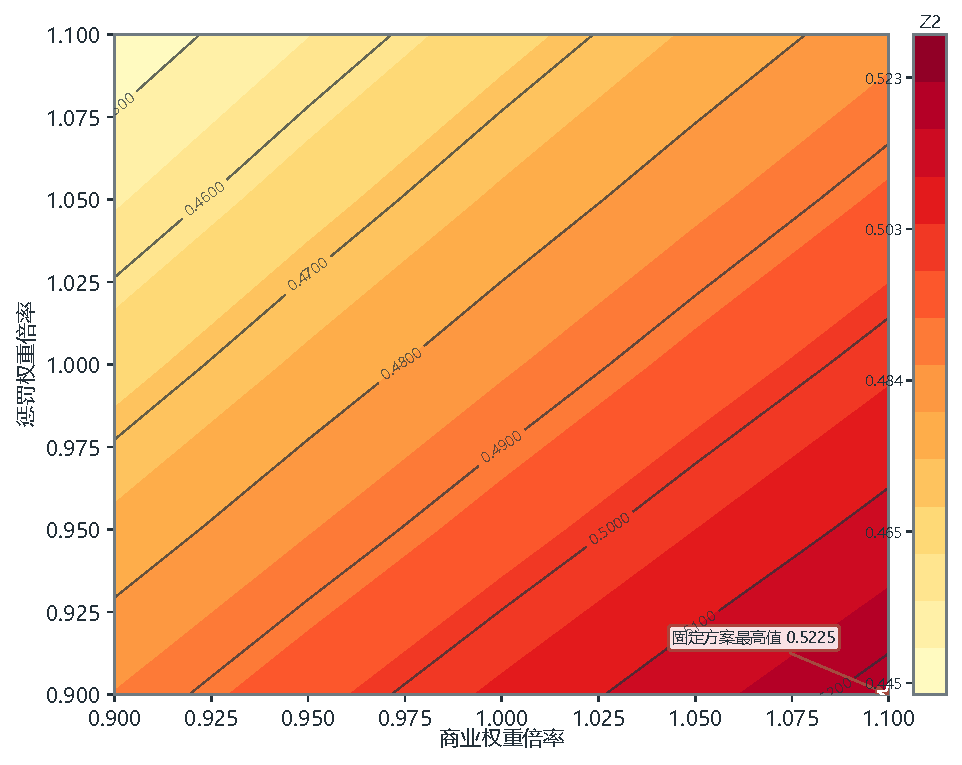
\includegraphics[width=0.85\textwidth,height=0.80\textheight,keepaspectratio]{../figures/fig_q2_weight_sensitivity_contour.pdf}
    \caption{问题二权重敏感性}
    \label{fig:q2-weight-sensitivity-contour}
\end{figure}

最大与最小得分之差为 $0.077041$，约占基准得分的 $15.9\%$，表明综合目标的绝对数值会随偏好改变，但没有出现符号异常或数量级失控。更重要的是，权重变化不改变问题二的硬约束：每队三场、场馆候选、相邻轮休息、日负荷和公平限制仍由同一组布尔变量与约束保证。因而，决策者可在这一曲面上选择偏好点，却不能把权重调整当作放松赛事规则的手段。

求解结果还经过独立的物理复算。$72$ 场均被唯一指派，最小相邻轮休息为 $63$ 小时，场馆负荷为 $2$ 至 $8$ 场，黄金时段次数极差为 $1$，大场馆次数极差为 $1$；全部硬约束无违反。求解器的 incumbent 为 $17811471$、best bound 为 $17883841$，按同一整数目标计算的证书间隙约 $0.41\%$，故应将其表述为满足设定 $0.5\%$ gap limit 的高质量解，而非零间隙证明。

\subsection{动态配置的参数灵敏度}

问题三分别将竞技状态系数和伤病系数乘以 $0.9,1.0,1.1$，形成 $3\times3$ 情景网格。每个情景都保持同一随机数流、共同信息截面、候选动作与日预算约束，并重新计算更新环境和动态最优动作。模型不含“改动惩罚”，因此该检验只衡量状态与伤病反馈参数对目标和资源组合的影响。

该参数网格下的 $Z_3$ 曲面见图\ref{fig:q3-sensitivity-surface}，取值在 $6.623009$ 至 $6.713491$ 之间变化，九个情景的平均晋级概率均为 $2/3$。曲面局部非单调，这是离散动作与日预算共同作用的结果；在所检验范围内没有出现目标数量级突变。

\begin{figure}[htbp]
    \centering
    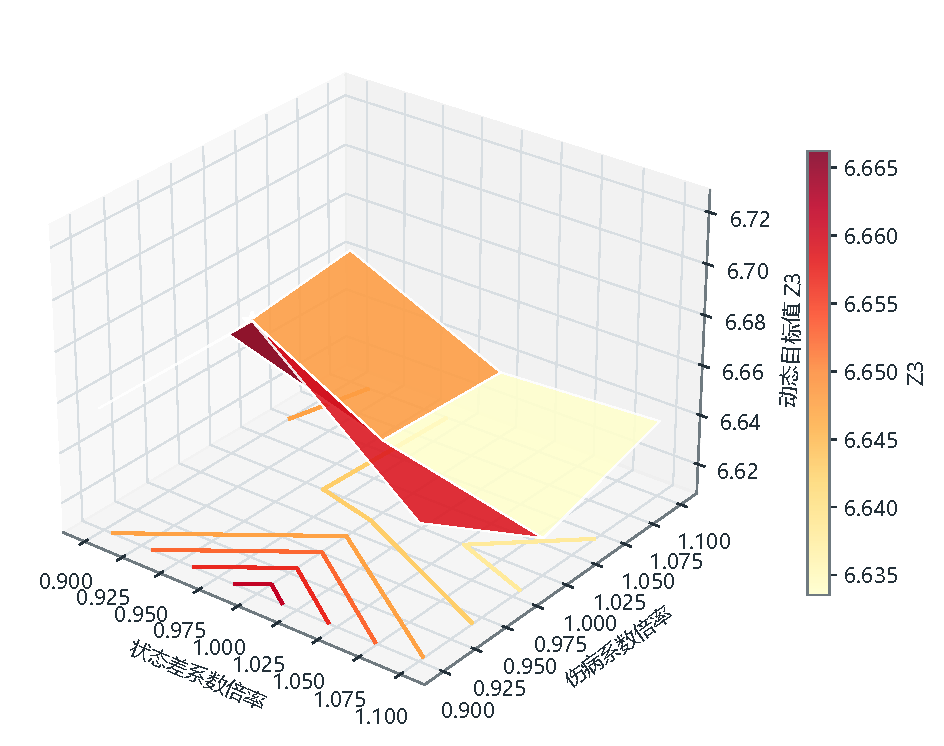
\includegraphics[width=0.85\textwidth,height=0.80\textheight,keepaspectratio]{../figures/fig_q3_sensitivity_surface.pdf}
    \caption{问题三参数敏感性}
    \label{fig:q3-sensitivity-surface}
\end{figure}

九点极差为 $0.090482$，相对中心量级约为 $1.4\%$。这说明动态目标值对所考察的参数扰动较稳定，但稳定并不意味着所有边界场次配置必然不变：基准情景已有 $8$ 场相对静态方案调档。实际执行时仍应把信息更新时间与赛事组织的通知周期共同设定，避免在资源已无法调整后才更新决策。

联合蒙特卡洛自身也经过重复性检验。五个随机种子下晋级概率标准差的最大值为 $0.004691$，且每个种子都重新构造更新环境并完整求解静态与动态资源模型。五次同界增益位于 $[0.065123,0.065434]$，四个附加种子的 $24$ 场动态决策均与基准完全一致，五次求解状态均为 \texttt{OPTIMAL}。因此稳定性不仅体现在边际概率，也落实到最终离散决策。

为避免三维曲面只给出视觉印象，表\ref{tab:q3-sensitivity-grid}列出九个参数点的完整目标值。状态系数倍率从 $0.9$ 增至 $1.1$ 并不保证 $Z_3$ 单调上升，因为动作集合是离散的，参数变化可能使少量边界比赛切换资源档位；伤病系数也通过双方状态、需求和风险共同作用。尽管局部存在非单调，九个点的晋级概率均值都保持 $2/3$，说明名额守恒没有被参数扰动破坏。

\begin{table}[htbp]
\centering
\caption{状态系数与伤病系数扰动下的$Z_3$}
\label{tab:q3-sensitivity-grid}
\begin{tabular}{cccc}
\toprule
状态倍率$\backslash$伤病倍率 & $0.9$ & $1.0$ & $1.1$ \\
\midrule
$0.9$ & 6.657086 & 6.656895 & 6.663519 \\
$1.0$ & 6.713491 & 6.637484 & 6.635101 \\
$1.1$ & 6.661416 & 6.623009 & 6.638511 \\
\bottomrule
\end{tabular}
\end{table}

最大值出现在状态倍率 $1.0$、伤病倍率 $0.9$，最小值出现在 $1.1$、$1.0$。二者并不位于同一参数方向的两个端点，说明目标差异来自离散资源组合与日预算共同形成的分段响应，而不是一个系数符号写反。实际部署若要扩大扰动范围，应在每个新参数点重新求解，不能用当前九点曲面作线性外推。

\subsection{现实比较的权重与代理检验}

问题四的权重扰动和代理扰动给出了不同层次的稳健性结论。在基准最近邻代理下，将八个权重分别上、下调 $10\%$ 后再归一化，共 $16$ 个情景，优化综合得分高于实际方案的方向保持率为 $100\%$。这表明基准方向不是由某个权重的局部微调所决定。

把实际比赛与场馆的全部代理从最近邻整体换成第二近邻后，实际方案得分由 $0.277058$ 变为 $0.226072$，优化方案仍为 $0.480778$，方向没有翻转。完整赛前 Elo、共同包络边界和唯一时段映射保证八项输入均位于 $[0,1]$。代理映射仍是主要不确定性来源，但在已检验邻居范围内不再改变条件性排序。

三种证据状态的对照汇总于表\ref{tab:q4-robustness-levels}。权重扰动下，实际代理分位于 $[0.267908,0.285763]$，优化分位于 $[0.469560,0.491449]$，二者区间不交叠；第二近邻整体替换后仍保持同向。结构层不依赖这些商业和安保邻居，其结论不随该替换改变。

\begin{table}[htbp]
\centering
\caption{问题四不同证据层的稳健性结果}
\label{tab:q4-robustness-levels}
\resizebox{\textwidth}{!}{%
\begin{tabular}{lccc}
\toprule
检验 & 实际赛程 & 优化赛程 & 允许的结论 \\
\midrule
基准最近邻 & 0.277058 & 0.480778 & 优化方向的条件性排序 \\
$16$个权重扰动 & 0.267908--0.285763 & 0.469560--0.491449 & 局部方向稳定 \\
第二近邻整体替换 & 0.226072 & 0.480778 & 邻居方向保持 \\
结构层复算 & 小时、公里、场馆日 & 同单位物理量 & 直接报告事实 \\
\bottomrule
\end{tabular}
}
\end{table}

这一区分说明“方向稳定”必须说明相对于哪一种扰动。权重检验只覆盖决策偏好的局部变化，第二近邻检验只覆盖一个局部代理替换；两者都不能代表真实合同和运营成本。现实 $48$ 场仍只映射到 $26$ 个题内比赛和 $4$ 个题内场馆，最高复用次数分别为 $6$ 和 $33$。只有结构层的来源与公式都能从逐场记录复核，因此其证据强度仍高于两个代理得分情景。

综合四问的检验结果可见，预测误差、权重偏好、状态反馈和代理映射属于四种不同的不确定性。前两类主要改变数值幅度，硬约束仍保持；第三类决定少量场次是否需要动态调档；第四类在已检验范围内未改变方向，却仍限制结论能否外推到真实运营。分层报告这些影响，比把所有扰动混合成一个“鲁棒性分数”更能说明模型的适用边界。

\section{正文补充图}

本附录保存正文因 30 页限制移出的探索性、流程性和解释性图。所有图均由本轮正式 JSON/CSV 重新生成。

\begin{figure}[htbp]
\centering
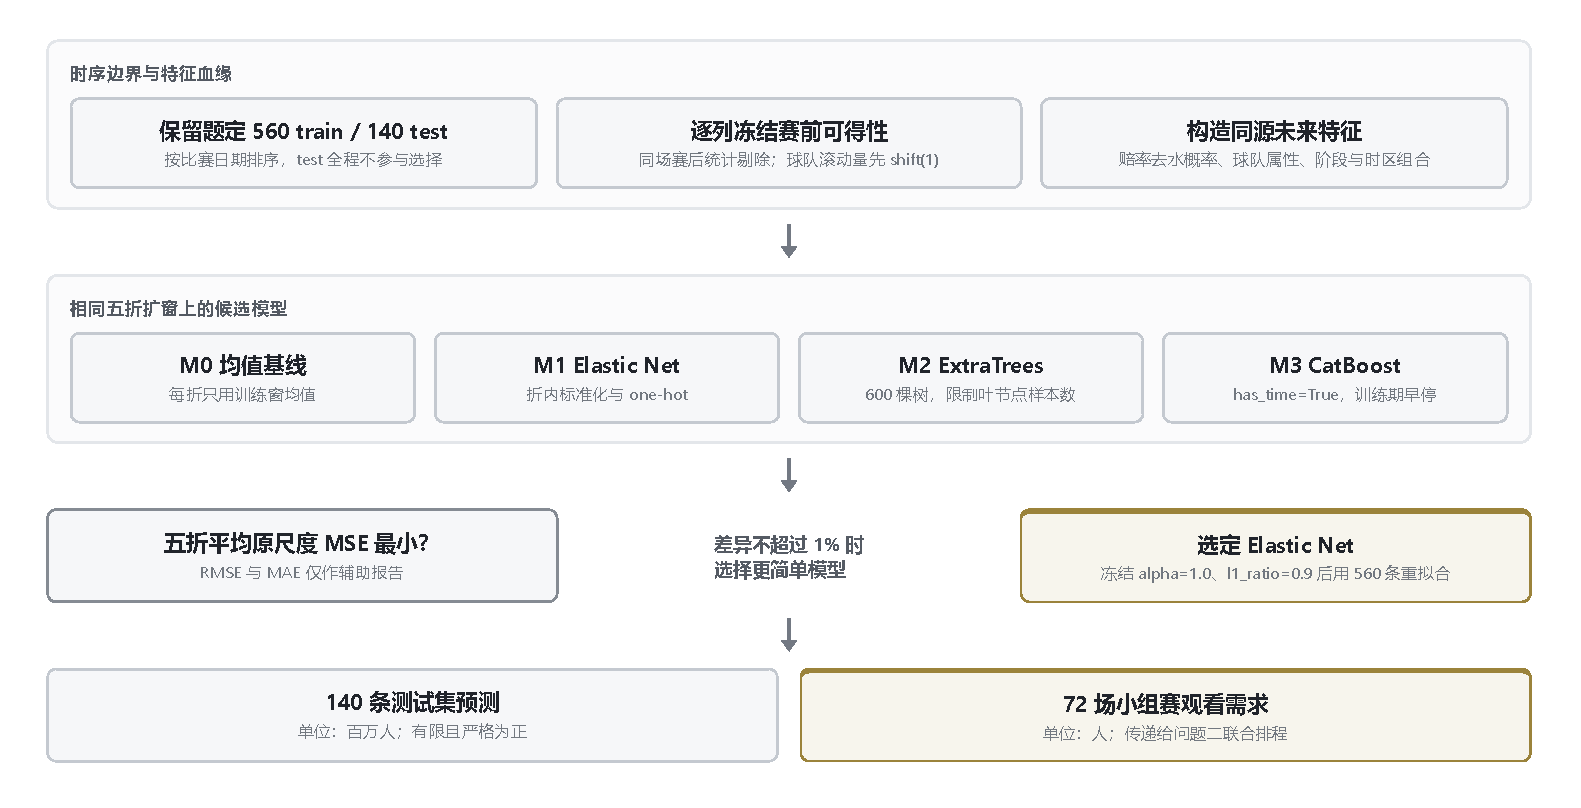
\includegraphics[width=0.85\textwidth,height=0.55\textheight,keepaspectratio]{../figures/fig_flow_q1.pdf}
\caption{问题一求解流程}\label{fig:flow-q1}
\end{figure}

\begin{figure}[htbp]
\centering
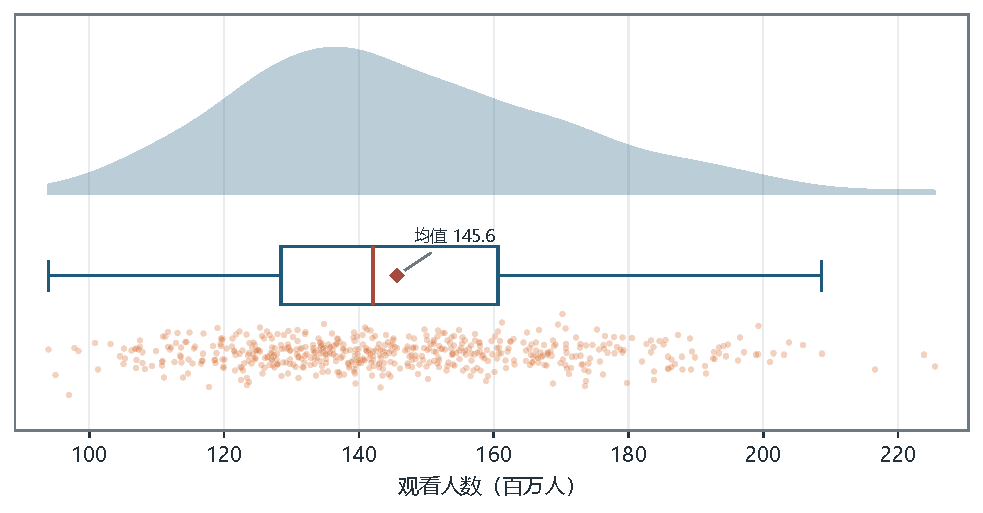
\includegraphics[width=0.85\textwidth,height=0.72\textheight,keepaspectratio]{../figures/fig_q1_target_raincloud.pdf}
\caption{训练集观看人数分布与长尾特征}\label{fig:q1-target-raincloud}
\end{figure}

\begin{figure}[htbp]
\centering
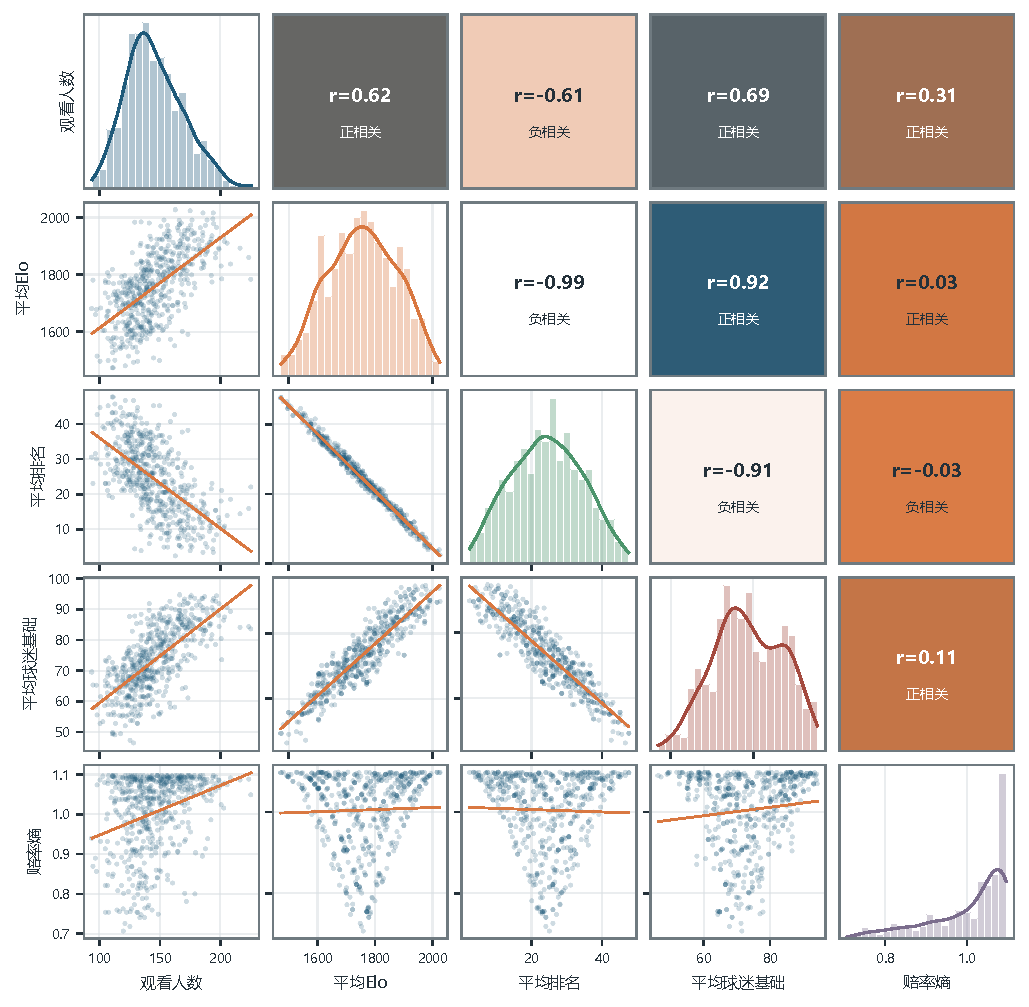
\includegraphics[width=0.85\textwidth,height=0.72\textheight,keepaspectratio]{../figures/fig_q1_feature_pairplot.pdf}
\caption{问题一核心赛前特征成对关系}\label{fig:q1-feature-pairplot}
\end{figure}

\begin{figure}[htbp]
\centering
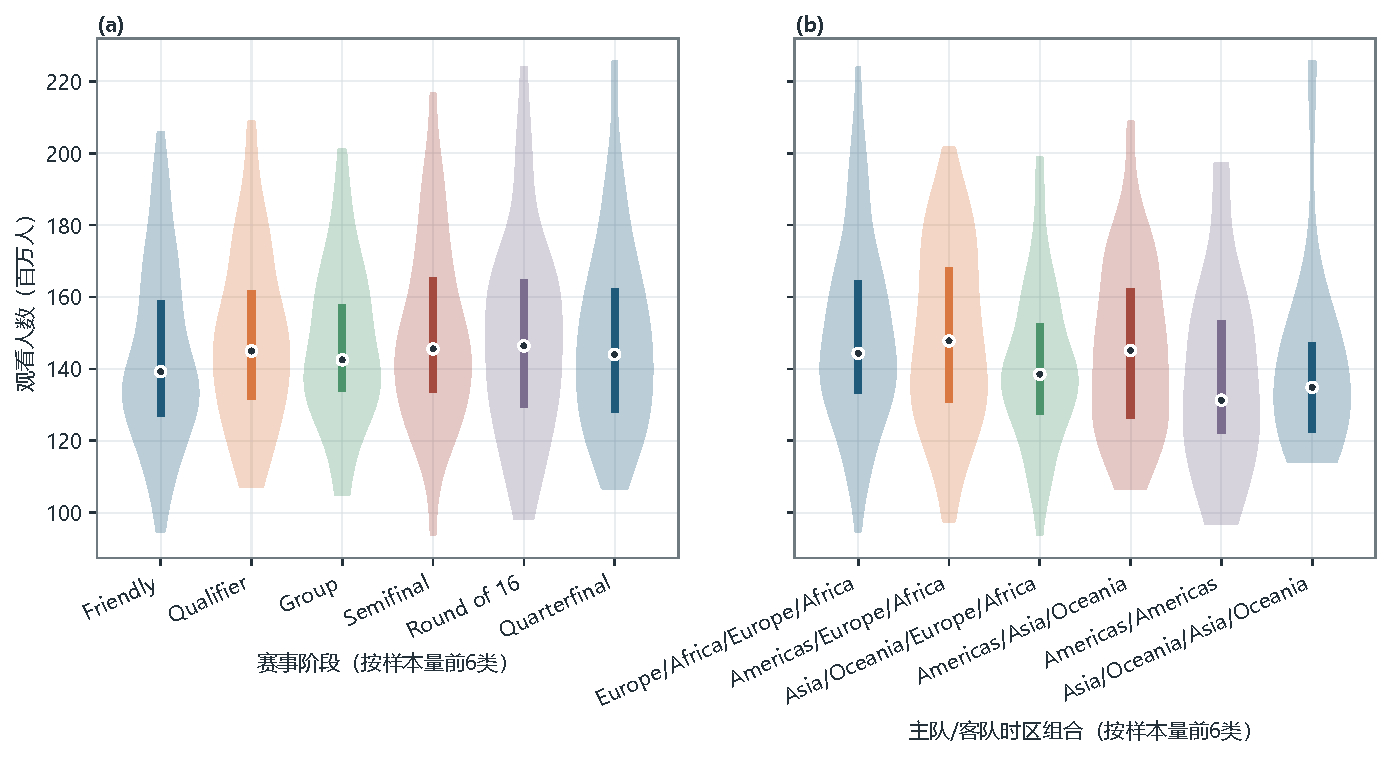
\includegraphics[width=0.85\textwidth,height=0.72\textheight,keepaspectratio]{../figures/fig_q1_stage_timezone_violin.pdf}
\caption{赛事阶段与时区组合下观看人数异质性}\label{fig:q1-stage-timezone-violin}
\end{figure}

\begin{figure}[htbp]
\centering
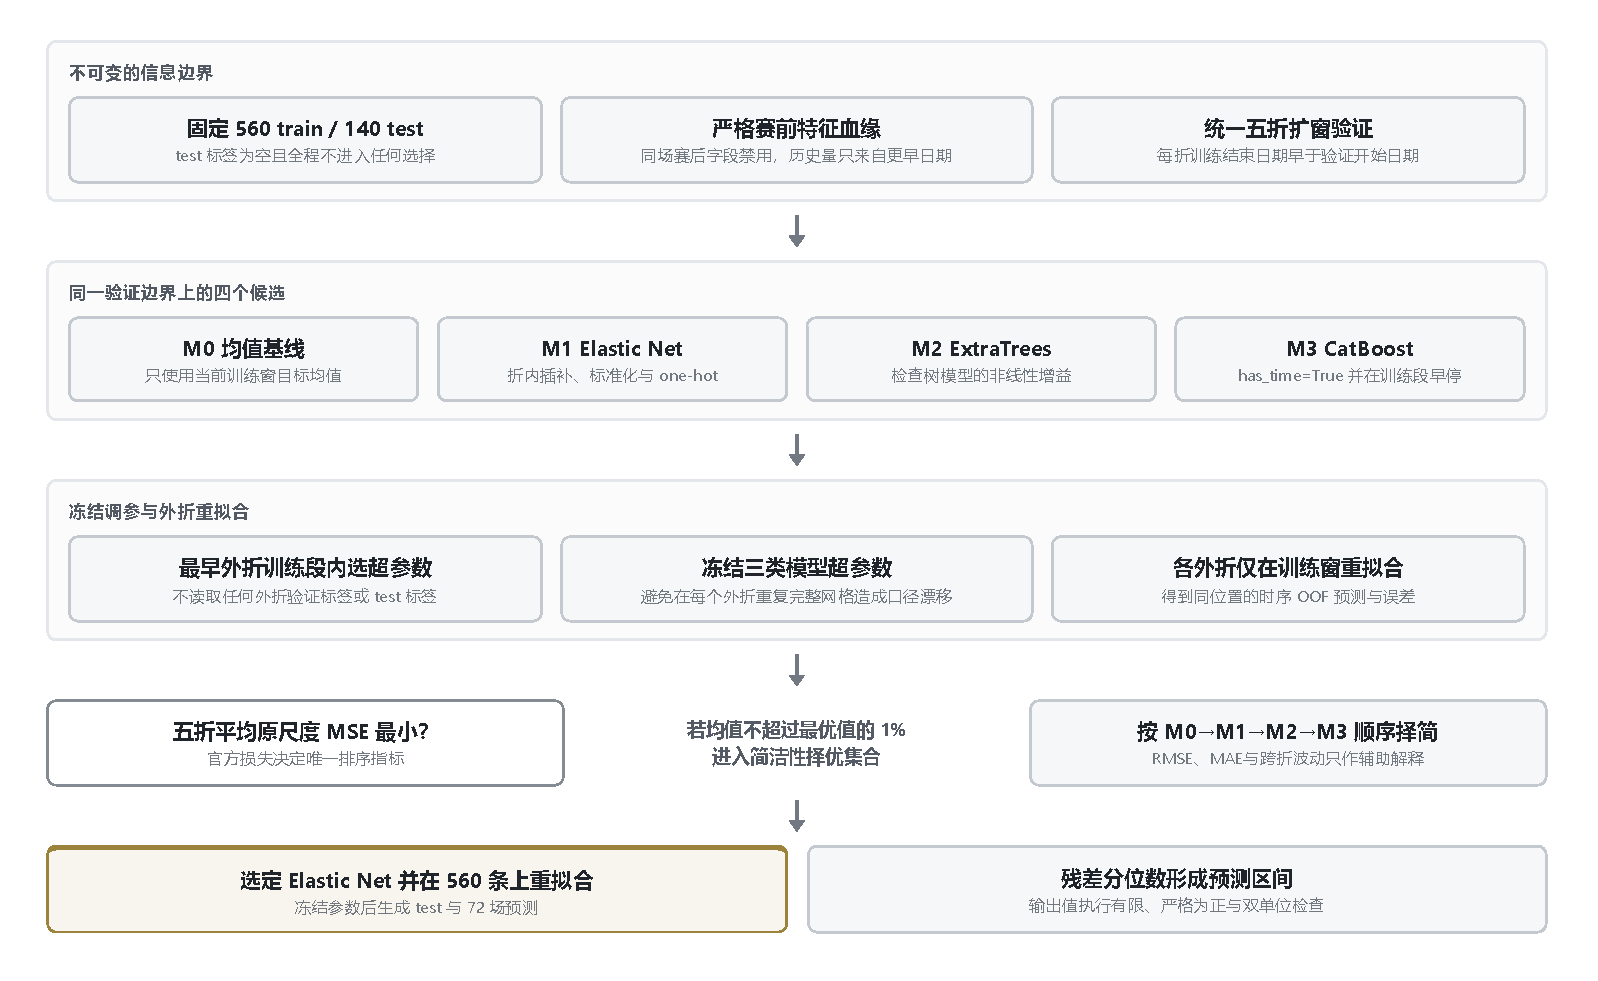
\includegraphics[width=0.85\textwidth,height=0.55\textheight,keepaspectratio]{../figures/fig_model_decision.pdf}
\caption{预测模型选择流程}\label{fig:model-decision}
\end{figure}

\begin{figure}[htbp]
\centering
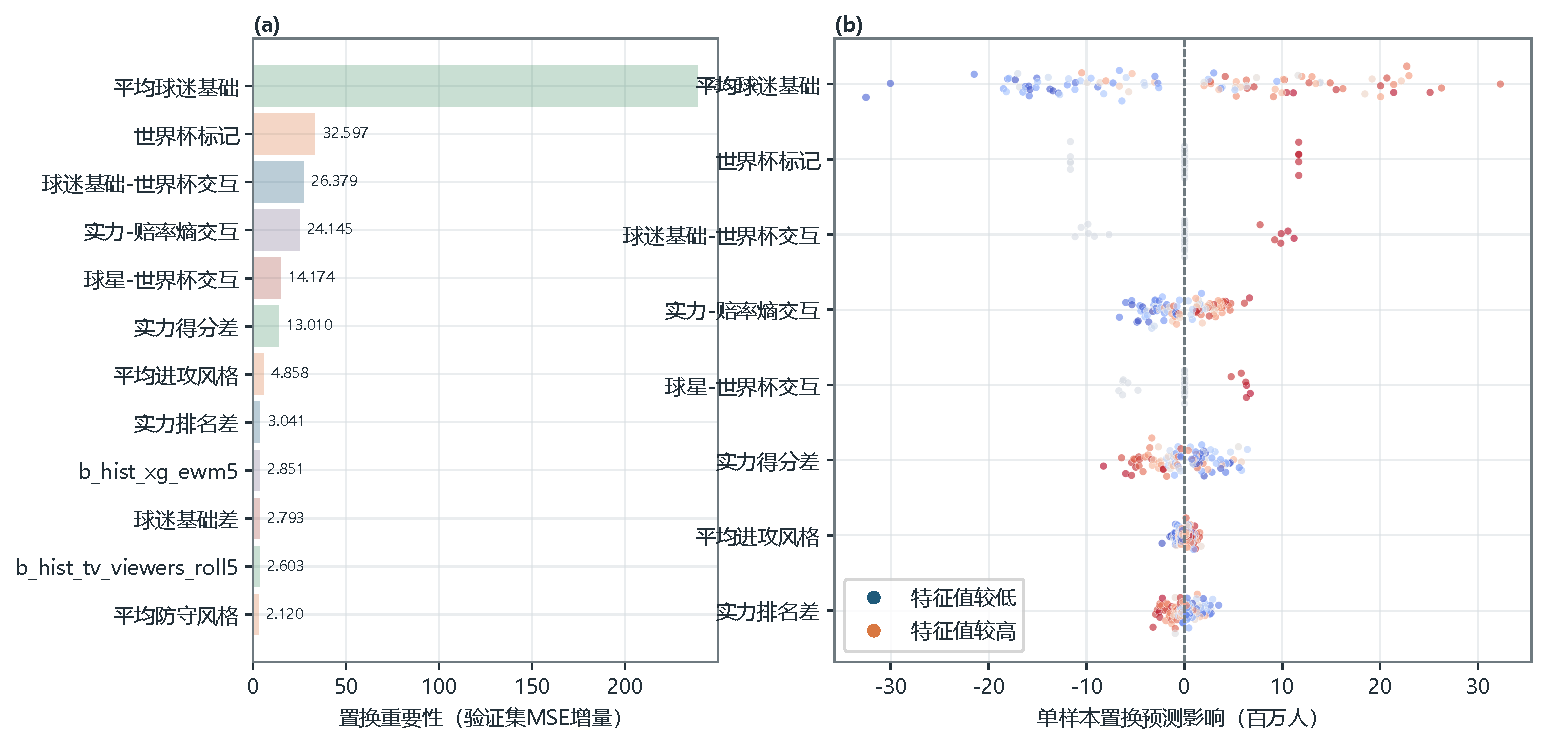
\includegraphics[width=0.85\textwidth,height=0.72\textheight,keepaspectratio]{../figures/fig_q1_shap_summary.pdf}
\caption{Elastic Net置换重要性与单样本预测影响}\label{fig:q1-shap-summary}
\end{figure}

\begin{figure}[htbp]
\centering
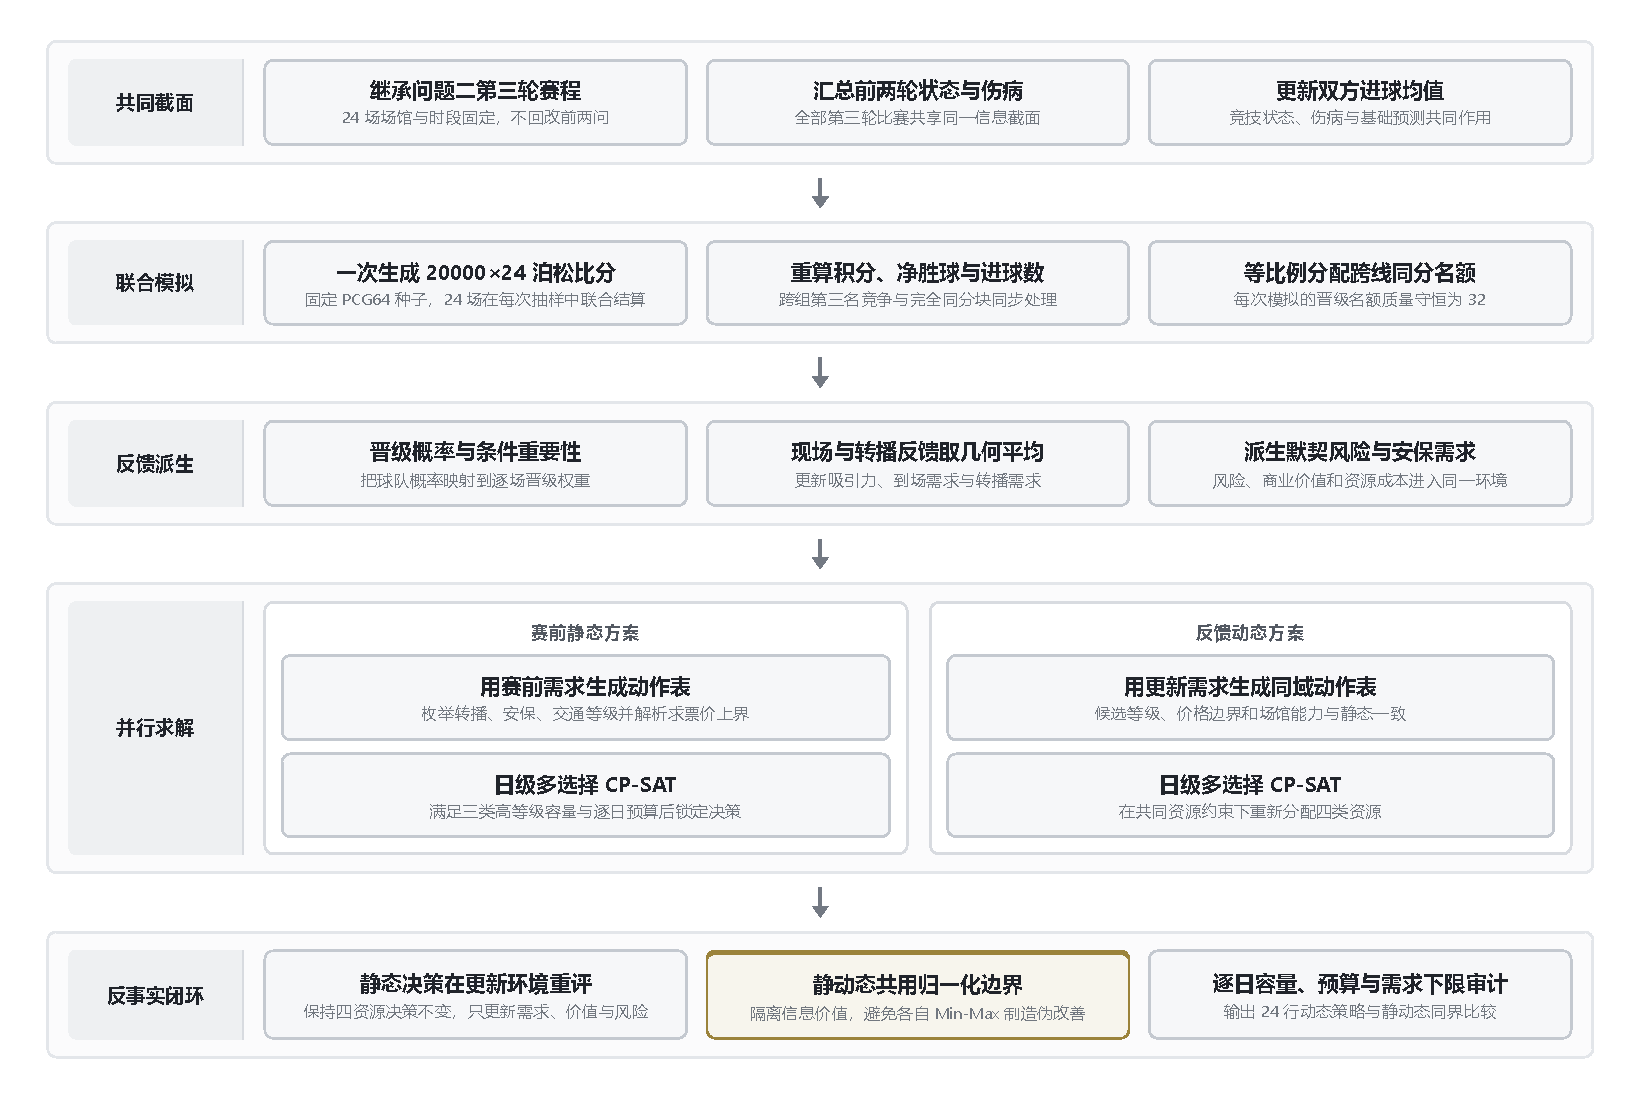
\includegraphics[width=0.88\textwidth,height=0.58\textheight,keepaspectratio]{../figures/fig_flow_q3.pdf}
\caption{问题三共同信息截面与静动态同界比较流程}\label{fig:flow-q3}
\end{figure}

\begin{figure}[htbp]
\centering
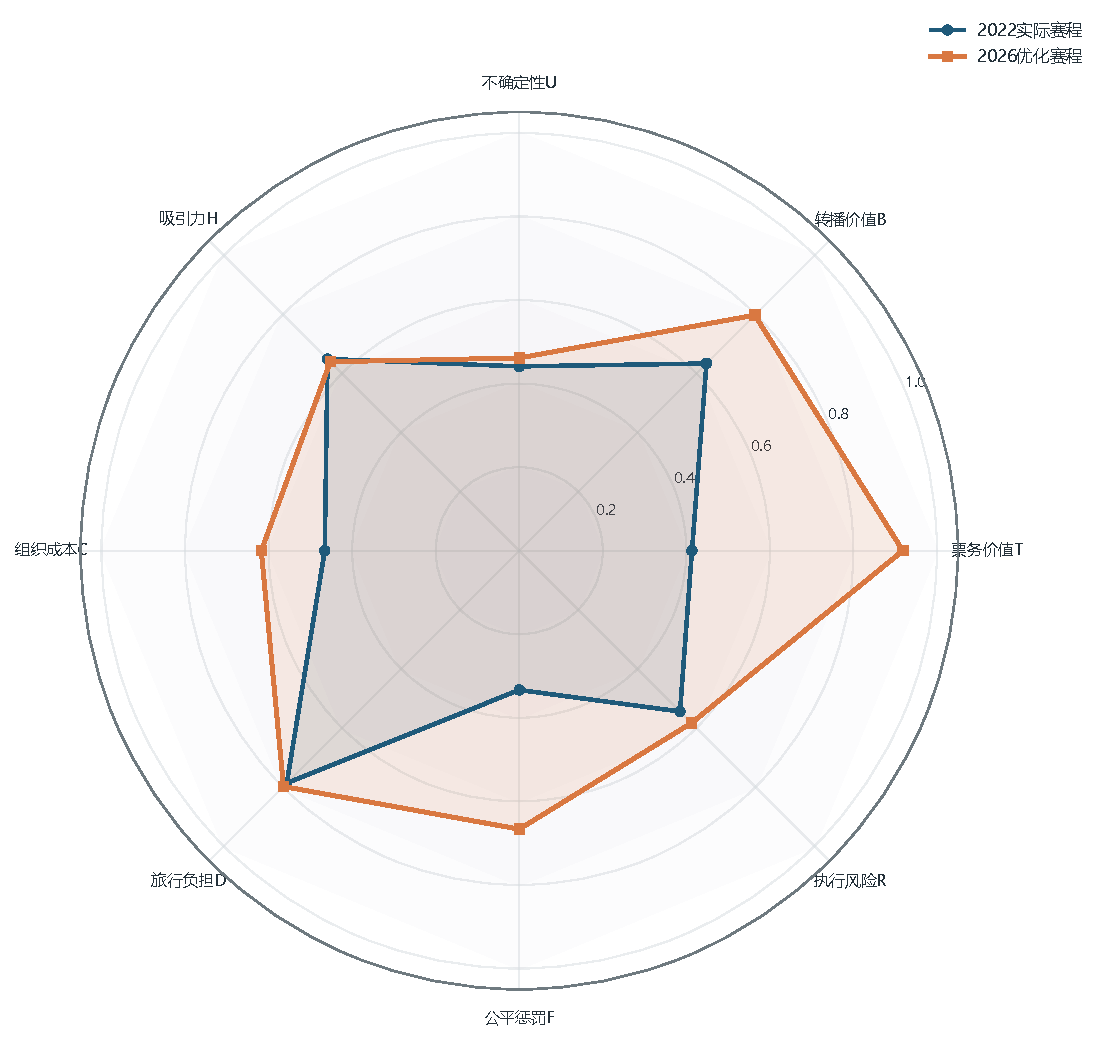
\includegraphics[width=0.85\textwidth,height=0.72\textheight,keepaspectratio]{../figures/fig_q4_metric_radar.pdf}
\caption{同构代理层的指标轮廓}\label{fig:q4-metric-radar}
\end{figure}

\section{支撑材料清单与完整源程序}

\subsection{支撑材料文件列表}

支撑材料压缩包采用如下目录结构；赛题提供的原始 Excel 不重复打包，复现时按 \texttt{README.md} 放入 \texttt{user\_data/} 即可。

\begin{longtable}{p{0.34\textwidth}p{0.60\textwidth}}
\toprule
路径 & 内容与用途 \\
\midrule
\endfirsthead
\toprule
路径 & 内容与用途 \\
\midrule
\endhead
\texttt{README.md} & 从空环境开始的安装、运行、输出和论文编译说明 \\
\texttt{requirements-lock.txt} & Python 3.12 的直接依赖精确版本 \\
\texttt{reproduce.py} & 四问、灵敏度、约束复核和图表的一键入口 \\
\texttt{code/} & 问题一至问题四、参数、工具、数据检查、灵敏度和约束复核的完整 Python 源码 \\
\texttt{figures/*.py}、\texttt{\_utils/} & 图表数据整理、统一绘图和 LaTeX 表格生成程序 \\
\texttt{paper/} & 论文 LaTeX 源文件、模板、字体、参考文献和已生成图表 \\
\texttt{output/} & 正式 CSV 及问题四可选比较输出的同内容副本 \\
\texttt{figures/problem\_*.json} & 四问完整机器结果、求解器状态、边界、审计和敏感性记录 \\
\path{user_data/worldcup_2022_openfootball.json} & 问题四真实赛程的机器读取快照 \\
\path{user_data/worldcup_2022_pre_tournament_elo.csv} & 问题四完整赛前 Elo 快照 \\
\texttt{actual\_schedule\_2022.csv} & 真实赛程逐场整理表、来源 URL 与访问日期 \\
\texttt{AI 工具使用详情.pdf} & 工具、用途、提示方式、采纳和核验记录 \\
\bottomrule
\end{longtable}

\subsection{完整结果附表}

以下附表由正式 JSON/CSV 直接生成，用于复核正文汇总值。

{
\footnotesize
\hfuzz=0.2pt
\setlength{\tabcolsep}{3pt}
\begin{longtable}{p{0.15\textwidth}p{0.16\textwidth}p{0.15\textwidth}p{0.18\textwidth}p{0.19\textwidth}}
\caption{问题一特征字典与时间血缘}\label{tab:q1-data-dictionary}\\
\toprule
特征 & 来源表 & 来源列 & 时间规则 & 拟合样本 \\
\midrule
\endfirsthead
\multicolumn{5}{c}{续表} \\
\toprule
特征 & 来源表 & 来源列 & 时间规则 & 拟合样本 \\
\midrule
\endhead
\midrule \multicolumn{5}{r}{续下页} \\
\endfoot
\bottomrule
\endlastfoot
competition & historical\_\allowbreak{}matches/\allowbreak{}teams/\allowbreak{}base\_\allowbreak{}predictions & competition & pregame\_\allowbreak{}available & outer\_\allowbreak{}fold\_\allowbreak{}train\_\allowbreak{}only;\allowbreak{} final=560 train ids \\
stage & historical\_\allowbreak{}matches/\allowbreak{}teams/\allowbreak{}base\_\allowbreak{}predictions & stage & pregame\_\allowbreak{}available & outer\_\allowbreak{}fold\_\allowbreak{}train\_\allowbreak{}only;\allowbreak{} final=560 train ids \\
timezone\_\allowbreak{}pair & historical\_\allowbreak{}matches/\allowbreak{}teams/\allowbreak{}base\_\allowbreak{}predictions & timezone\_\allowbreak{}pair & pregame\_\allowbreak{}available & outer\_\allowbreak{}fold\_\allowbreak{}train\_\allowbreak{}only;\allowbreak{} final=560 train ids \\
strength\_\allowbreak{}rank\_\allowbreak{}mean & historical\_\allowbreak{}matches/\allowbreak{}teams/\allowbreak{}base\_\allowbreak{}predictions & strength\_\allowbreak{}rank\_\allowbreak{}mean & pregame\_\allowbreak{}available & outer\_\allowbreak{}fold\_\allowbreak{}train\_\allowbreak{}only;\allowbreak{} final=560 train ids \\
strength\_\allowbreak{}rank\_\allowbreak{}gap & historical\_\allowbreak{}matches/\allowbreak{}teams/\allowbreak{}base\_\allowbreak{}predictions & strength\_\allowbreak{}rank\_\allowbreak{}gap & pregame\_\allowbreak{}available & outer\_\allowbreak{}fold\_\allowbreak{}train\_\allowbreak{}only;\allowbreak{} final=560 train ids \\
elo\_\allowbreak{}mean & historical\_\allowbreak{}matches/\allowbreak{}teams/\allowbreak{}base\_\allowbreak{}predictions & elo\_\allowbreak{}mean & pregame\_\allowbreak{}available & outer\_\allowbreak{}fold\_\allowbreak{}train\_\allowbreak{}only;\allowbreak{} final=560 train ids \\
elo\_\allowbreak{}gap & historical\_\allowbreak{}matches/\allowbreak{}teams/\allowbreak{}base\_\allowbreak{}predictions & elo\_\allowbreak{}gap & pregame\_\allowbreak{}available & outer\_\allowbreak{}fold\_\allowbreak{}train\_\allowbreak{}only;\allowbreak{} final=560 train ids \\
p\_\allowbreak{}a & historical\_\allowbreak{}matches/\allowbreak{}teams/\allowbreak{}base\_\allowbreak{}predictions & p\_\allowbreak{}a & pregame\_\allowbreak{}available & outer\_\allowbreak{}fold\_\allowbreak{}train\_\allowbreak{}only;\allowbreak{} final=560 train ids \\
p\_\allowbreak{}draw & historical\_\allowbreak{}matches/\allowbreak{}teams/\allowbreak{}base\_\allowbreak{}predictions & p\_\allowbreak{}draw & pregame\_\allowbreak{}available & outer\_\allowbreak{}fold\_\allowbreak{}train\_\allowbreak{}only;\allowbreak{} final=560 train ids \\
p\_\allowbreak{}b & historical\_\allowbreak{}matches/\allowbreak{}teams/\allowbreak{}base\_\allowbreak{}predictions & p\_\allowbreak{}b & pregame\_\allowbreak{}available & outer\_\allowbreak{}fold\_\allowbreak{}train\_\allowbreak{}only;\allowbreak{} final=560 train ids \\
odds\_\allowbreak{}entropy & historical\_\allowbreak{}matches/\allowbreak{}teams/\allowbreak{}base\_\allowbreak{}predictions & odds\_\allowbreak{}entropy & pregame\_\allowbreak{}available & outer\_\allowbreak{}fold\_\allowbreak{}train\_\allowbreak{}only;\allowbreak{} final=560 train ids \\
market\_\allowbreak{}value\_\allowbreak{}musd\_\allowbreak{}mean & historical\_\allowbreak{}matches/\allowbreak{}teams/\allowbreak{}base\_\allowbreak{}predictions & market\_\allowbreak{}value\_\allowbreak{}musd\_\allowbreak{}mean & pregame\_\allowbreak{}available & outer\_\allowbreak{}fold\_\allowbreak{}train\_\allowbreak{}only;\allowbreak{} final=560 train ids \\
market\_\allowbreak{}value\_\allowbreak{}musd\_\allowbreak{}gap & historical\_\allowbreak{}matches/\allowbreak{}teams/\allowbreak{}base\_\allowbreak{}predictions & market\_\allowbreak{}value\_\allowbreak{}musd\_\allowbreak{}gap & pregame\_\allowbreak{}available & outer\_\allowbreak{}fold\_\allowbreak{}train\_\allowbreak{}only;\allowbreak{} final=560 train ids \\
avg\_\allowbreak{}age\_\allowbreak{}mean & historical\_\allowbreak{}matches/\allowbreak{}teams/\allowbreak{}base\_\allowbreak{}predictions & avg\_\allowbreak{}age\_\allowbreak{}mean & pregame\_\allowbreak{}available & outer\_\allowbreak{}fold\_\allowbreak{}train\_\allowbreak{}only;\allowbreak{} final=560 train ids \\
avg\_\allowbreak{}age\_\allowbreak{}gap & historical\_\allowbreak{}matches/\allowbreak{}teams/\allowbreak{}base\_\allowbreak{}predictions & avg\_\allowbreak{}age\_\allowbreak{}gap & pregame\_\allowbreak{}available & outer\_\allowbreak{}fold\_\allowbreak{}train\_\allowbreak{}only;\allowbreak{} final=560 train ids \\
star\_\allowbreak{}index\_\allowbreak{}mean & historical\_\allowbreak{}matches/\allowbreak{}teams/\allowbreak{}base\_\allowbreak{}predictions & star\_\allowbreak{}index\_\allowbreak{}mean & pregame\_\allowbreak{}available & outer\_\allowbreak{}fold\_\allowbreak{}train\_\allowbreak{}only;\allowbreak{} final=560 train ids \\
star\_\allowbreak{}index\_\allowbreak{}gap & historical\_\allowbreak{}matches/\allowbreak{}teams/\allowbreak{}base\_\allowbreak{}predictions & star\_\allowbreak{}index\_\allowbreak{}gap & pregame\_\allowbreak{}available & outer\_\allowbreak{}fold\_\allowbreak{}train\_\allowbreak{}only;\allowbreak{} final=560 train ids \\
fan\_\allowbreak{}base\_\allowbreak{}index\_\allowbreak{}mean & historical\_\allowbreak{}matches/\allowbreak{}teams/\allowbreak{}base\_\allowbreak{}predictions & fan\_\allowbreak{}base\_\allowbreak{}index\_\allowbreak{}mean & pregame\_\allowbreak{}available & outer\_\allowbreak{}fold\_\allowbreak{}train\_\allowbreak{}only;\allowbreak{} final=560 train ids \\
fan\_\allowbreak{}base\_\allowbreak{}index\_\allowbreak{}gap & historical\_\allowbreak{}matches/\allowbreak{}teams/\allowbreak{}base\_\allowbreak{}predictions & fan\_\allowbreak{}base\_\allowbreak{}index\_\allowbreak{}gap & pregame\_\allowbreak{}available & outer\_\allowbreak{}fold\_\allowbreak{}train\_\allowbreak{}only;\allowbreak{} final=560 train ids \\
style\_\allowbreak{}attack\_\allowbreak{}mean & historical\_\allowbreak{}matches/\allowbreak{}teams/\allowbreak{}base\_\allowbreak{}predictions & style\_\allowbreak{}attack\_\allowbreak{}mean & pregame\_\allowbreak{}available & outer\_\allowbreak{}fold\_\allowbreak{}train\_\allowbreak{}only;\allowbreak{} final=560 train ids \\
style\_\allowbreak{}attack\_\allowbreak{}gap & historical\_\allowbreak{}matches/\allowbreak{}teams/\allowbreak{}base\_\allowbreak{}predictions & style\_\allowbreak{}attack\_\allowbreak{}gap & pregame\_\allowbreak{}available & outer\_\allowbreak{}fold\_\allowbreak{}train\_\allowbreak{}only;\allowbreak{} final=560 train ids \\
style\_\allowbreak{}defense\_\allowbreak{}mean & historical\_\allowbreak{}matches/\allowbreak{}teams/\allowbreak{}base\_\allowbreak{}predictions & style\_\allowbreak{}defense\_\allowbreak{}mean & pregame\_\allowbreak{}available & outer\_\allowbreak{}fold\_\allowbreak{}train\_\allowbreak{}only;\allowbreak{} final=560 train ids \\
style\_\allowbreak{}defense\_\allowbreak{}gap & historical\_\allowbreak{}matches/\allowbreak{}teams/\allowbreak{}base\_\allowbreak{}predictions & style\_\allowbreak{}defense\_\allowbreak{}gap & pregame\_\allowbreak{}available & outer\_\allowbreak{}fold\_\allowbreak{}train\_\allowbreak{}only;\allowbreak{} final=560 train ids \\
host\_\allowbreak{}flag\_\allowbreak{}mean & historical\_\allowbreak{}matches/\allowbreak{}teams/\allowbreak{}base\_\allowbreak{}predictions & host\_\allowbreak{}flag\_\allowbreak{}mean & pregame\_\allowbreak{}available & outer\_\allowbreak{}fold\_\allowbreak{}train\_\allowbreak{}only;\allowbreak{} final=560 train ids \\
host\_\allowbreak{}flag\_\allowbreak{}gap & historical\_\allowbreak{}matches/\allowbreak{}teams/\allowbreak{}base\_\allowbreak{}predictions & host\_\allowbreak{}flag\_\allowbreak{}gap & pregame\_\allowbreak{}available & outer\_\allowbreak{}fold\_\allowbreak{}train\_\allowbreak{}only;\allowbreak{} final=560 train ids \\
strength\_\allowbreak{}score\_\allowbreak{}mean & historical\_\allowbreak{}matches/\allowbreak{}teams/\allowbreak{}base\_\allowbreak{}predictions & strength\_\allowbreak{}score\_\allowbreak{}mean & pregame\_\allowbreak{}available & outer\_\allowbreak{}fold\_\allowbreak{}train\_\allowbreak{}only;\allowbreak{} final=560 train ids \\
strength\_\allowbreak{}score\_\allowbreak{}gap & historical\_\allowbreak{}matches/\allowbreak{}teams/\allowbreak{}base\_\allowbreak{}predictions & strength\_\allowbreak{}score\_\allowbreak{}gap & pregame\_\allowbreak{}available & outer\_\allowbreak{}fold\_\allowbreak{}train\_\allowbreak{}only;\allowbreak{} final=560 train ids \\
a\_\allowbreak{}hist\_\allowbreak{}goals\_\allowbreak{}roll5 & historical\_\allowbreak{}matches & a\_\allowbreak{}hist\_\allowbreak{}goals\_\allowbreak{}roll5 & strictly\_\allowbreak{}before\_\allowbreak{}kickoff\_\allowbreak{}shift1 & outer\_\allowbreak{}fold\_\allowbreak{}train\_\allowbreak{}only;\allowbreak{} final=560 train ids \\
a\_\allowbreak{}hist\_\allowbreak{}goals\_\allowbreak{}ewm5 & historical\_\allowbreak{}matches & a\_\allowbreak{}hist\_\allowbreak{}goals\_\allowbreak{}ewm5 & strictly\_\allowbreak{}before\_\allowbreak{}kickoff\_\allowbreak{}shift1 & outer\_\allowbreak{}fold\_\allowbreak{}train\_\allowbreak{}only;\allowbreak{} final=560 train ids \\
a\_\allowbreak{}hist\_\allowbreak{}xg\_\allowbreak{}roll5 & historical\_\allowbreak{}matches & a\_\allowbreak{}hist\_\allowbreak{}xg\_\allowbreak{}roll5 & strictly\_\allowbreak{}before\_\allowbreak{}kickoff\_\allowbreak{}shift1 & outer\_\allowbreak{}fold\_\allowbreak{}train\_\allowbreak{}only;\allowbreak{} final=560 train ids \\
a\_\allowbreak{}hist\_\allowbreak{}xg\_\allowbreak{}ewm5 & historical\_\allowbreak{}matches & a\_\allowbreak{}hist\_\allowbreak{}xg\_\allowbreak{}ewm5 & strictly\_\allowbreak{}before\_\allowbreak{}kickoff\_\allowbreak{}shift1 & outer\_\allowbreak{}fold\_\allowbreak{}train\_\allowbreak{}only;\allowbreak{} final=560 train ids \\
a\_\allowbreak{}hist\_\allowbreak{}shots\_\allowbreak{}roll5 & historical\_\allowbreak{}matches & a\_\allowbreak{}hist\_\allowbreak{}shots\_\allowbreak{}roll5 & strictly\_\allowbreak{}before\_\allowbreak{}kickoff\_\allowbreak{}shift1 & outer\_\allowbreak{}fold\_\allowbreak{}train\_\allowbreak{}only;\allowbreak{} final=560 train ids \\
a\_\allowbreak{}hist\_\allowbreak{}shots\_\allowbreak{}ewm5 & historical\_\allowbreak{}matches & a\_\allowbreak{}hist\_\allowbreak{}shots\_\allowbreak{}ewm5 & strictly\_\allowbreak{}before\_\allowbreak{}kickoff\_\allowbreak{}shift1 & outer\_\allowbreak{}fold\_\allowbreak{}train\_\allowbreak{}only;\allowbreak{} final=560 train ids \\
a\_\allowbreak{}hist\_\allowbreak{}possession\_\allowbreak{}roll5 & historical\_\allowbreak{}matches & a\_\allowbreak{}hist\_\allowbreak{}possession\_\allowbreak{}roll5 & strictly\_\allowbreak{}before\_\allowbreak{}kickoff\_\allowbreak{}shift1 & outer\_\allowbreak{}fold\_\allowbreak{}train\_\allowbreak{}only;\allowbreak{} final=560 train ids \\
a\_\allowbreak{}hist\_\allowbreak{}possession\_\allowbreak{}ewm5 & historical\_\allowbreak{}matches & a\_\allowbreak{}hist\_\allowbreak{}possession\_\allowbreak{}ewm5 & strictly\_\allowbreak{}before\_\allowbreak{}kickoff\_\allowbreak{}shift1 & outer\_\allowbreak{}fold\_\allowbreak{}train\_\allowbreak{}only;\allowbreak{} final=560 train ids \\
a\_\allowbreak{}hist\_\allowbreak{}attendance\_\allowbreak{}roll5 & historical\_\allowbreak{}matches & a\_\allowbreak{}hist\_\allowbreak{}attendance\_\allowbreak{}roll5 & strictly\_\allowbreak{}before\_\allowbreak{}kickoff\_\allowbreak{}shift1 & outer\_\allowbreak{}fold\_\allowbreak{}train\_\allowbreak{}only;\allowbreak{} final=560 train ids \\
a\_\allowbreak{}hist\_\allowbreak{}attendance\_\allowbreak{}ewm5 & historical\_\allowbreak{}matches & a\_\allowbreak{}hist\_\allowbreak{}attendance\_\allowbreak{}ewm5 & strictly\_\allowbreak{}before\_\allowbreak{}kickoff\_\allowbreak{}shift1 & outer\_\allowbreak{}fold\_\allowbreak{}train\_\allowbreak{}only;\allowbreak{} final=560 train ids \\
a\_\allowbreak{}hist\_\allowbreak{}tv\_\allowbreak{}viewers\_\allowbreak{}roll5 & historical\_\allowbreak{}matches & a\_\allowbreak{}hist\_\allowbreak{}tv\_\allowbreak{}viewers\_\allowbreak{}roll5 & strictly\_\allowbreak{}before\_\allowbreak{}kickoff\_\allowbreak{}shift1 & outer\_\allowbreak{}fold\_\allowbreak{}train\_\allowbreak{}only;\allowbreak{} final=560 train ids \\
a\_\allowbreak{}hist\_\allowbreak{}tv\_\allowbreak{}viewers\_\allowbreak{}ewm5 & historical\_\allowbreak{}matches & a\_\allowbreak{}hist\_\allowbreak{}tv\_\allowbreak{}viewers\_\allowbreak{}ewm5 & strictly\_\allowbreak{}before\_\allowbreak{}kickoff\_\allowbreak{}shift1 & outer\_\allowbreak{}fold\_\allowbreak{}train\_\allowbreak{}only;\allowbreak{} final=560 train ids \\
b\_\allowbreak{}hist\_\allowbreak{}goals\_\allowbreak{}roll5 & historical\_\allowbreak{}matches & b\_\allowbreak{}hist\_\allowbreak{}goals\_\allowbreak{}roll5 & strictly\_\allowbreak{}before\_\allowbreak{}kickoff\_\allowbreak{}shift1 & outer\_\allowbreak{}fold\_\allowbreak{}train\_\allowbreak{}only;\allowbreak{} final=560 train ids \\
b\_\allowbreak{}hist\_\allowbreak{}goals\_\allowbreak{}ewm5 & historical\_\allowbreak{}matches & b\_\allowbreak{}hist\_\allowbreak{}goals\_\allowbreak{}ewm5 & strictly\_\allowbreak{}before\_\allowbreak{}kickoff\_\allowbreak{}shift1 & outer\_\allowbreak{}fold\_\allowbreak{}train\_\allowbreak{}only;\allowbreak{} final=560 train ids \\
b\_\allowbreak{}hist\_\allowbreak{}xg\_\allowbreak{}roll5 & historical\_\allowbreak{}matches & b\_\allowbreak{}hist\_\allowbreak{}xg\_\allowbreak{}roll5 & strictly\_\allowbreak{}before\_\allowbreak{}kickoff\_\allowbreak{}shift1 & outer\_\allowbreak{}fold\_\allowbreak{}train\_\allowbreak{}only;\allowbreak{} final=560 train ids \\
b\_\allowbreak{}hist\_\allowbreak{}xg\_\allowbreak{}ewm5 & historical\_\allowbreak{}matches & b\_\allowbreak{}hist\_\allowbreak{}xg\_\allowbreak{}ewm5 & strictly\_\allowbreak{}before\_\allowbreak{}kickoff\_\allowbreak{}shift1 & outer\_\allowbreak{}fold\_\allowbreak{}train\_\allowbreak{}only;\allowbreak{} final=560 train ids \\
b\_\allowbreak{}hist\_\allowbreak{}shots\_\allowbreak{}roll5 & historical\_\allowbreak{}matches & b\_\allowbreak{}hist\_\allowbreak{}shots\_\allowbreak{}roll5 & strictly\_\allowbreak{}before\_\allowbreak{}kickoff\_\allowbreak{}shift1 & outer\_\allowbreak{}fold\_\allowbreak{}train\_\allowbreak{}only;\allowbreak{} final=560 train ids \\
b\_\allowbreak{}hist\_\allowbreak{}shots\_\allowbreak{}ewm5 & historical\_\allowbreak{}matches & b\_\allowbreak{}hist\_\allowbreak{}shots\_\allowbreak{}ewm5 & strictly\_\allowbreak{}before\_\allowbreak{}kickoff\_\allowbreak{}shift1 & outer\_\allowbreak{}fold\_\allowbreak{}train\_\allowbreak{}only;\allowbreak{} final=560 train ids \\
b\_\allowbreak{}hist\_\allowbreak{}possession\_\allowbreak{}roll5 & historical\_\allowbreak{}matches & b\_\allowbreak{}hist\_\allowbreak{}possession\_\allowbreak{}roll5 & strictly\_\allowbreak{}before\_\allowbreak{}kickoff\_\allowbreak{}shift1 & outer\_\allowbreak{}fold\_\allowbreak{}train\_\allowbreak{}only;\allowbreak{} final=560 train ids \\
b\_\allowbreak{}hist\_\allowbreak{}possession\_\allowbreak{}ewm5 & historical\_\allowbreak{}matches & b\_\allowbreak{}hist\_\allowbreak{}possession\_\allowbreak{}ewm5 & strictly\_\allowbreak{}before\_\allowbreak{}kickoff\_\allowbreak{}shift1 & outer\_\allowbreak{}fold\_\allowbreak{}train\_\allowbreak{}only;\allowbreak{} final=560 train ids \\
b\_\allowbreak{}hist\_\allowbreak{}attendance\_\allowbreak{}roll5 & historical\_\allowbreak{}matches & b\_\allowbreak{}hist\_\allowbreak{}attendance\_\allowbreak{}roll5 & strictly\_\allowbreak{}before\_\allowbreak{}kickoff\_\allowbreak{}shift1 & outer\_\allowbreak{}fold\_\allowbreak{}train\_\allowbreak{}only;\allowbreak{} final=560 train ids \\
b\_\allowbreak{}hist\_\allowbreak{}attendance\_\allowbreak{}ewm5 & historical\_\allowbreak{}matches & b\_\allowbreak{}hist\_\allowbreak{}attendance\_\allowbreak{}ewm5 & strictly\_\allowbreak{}before\_\allowbreak{}kickoff\_\allowbreak{}shift1 & outer\_\allowbreak{}fold\_\allowbreak{}train\_\allowbreak{}only;\allowbreak{} final=560 train ids \\
b\_\allowbreak{}hist\_\allowbreak{}tv\_\allowbreak{}viewers\_\allowbreak{}roll5 & historical\_\allowbreak{}matches & b\_\allowbreak{}hist\_\allowbreak{}tv\_\allowbreak{}viewers\_\allowbreak{}roll5 & strictly\_\allowbreak{}before\_\allowbreak{}kickoff\_\allowbreak{}shift1 & outer\_\allowbreak{}fold\_\allowbreak{}train\_\allowbreak{}only;\allowbreak{} final=560 train ids \\
b\_\allowbreak{}hist\_\allowbreak{}tv\_\allowbreak{}viewers\_\allowbreak{}ewm5 & historical\_\allowbreak{}matches & b\_\allowbreak{}hist\_\allowbreak{}tv\_\allowbreak{}viewers\_\allowbreak{}ewm5 & strictly\_\allowbreak{}before\_\allowbreak{}kickoff\_\allowbreak{}shift1 & outer\_\allowbreak{}fold\_\allowbreak{}train\_\allowbreak{}only;\allowbreak{} final=560 train ids \\
worldcup\_\allowbreak{}stage & historical\_\allowbreak{}matches/\allowbreak{}teams/\allowbreak{}base\_\allowbreak{}predictions & worldcup\_\allowbreak{}stage & pregame\_\allowbreak{}available & outer\_\allowbreak{}fold\_\allowbreak{}train\_\allowbreak{}only;\allowbreak{} final=560 train ids \\
fan\_\allowbreak{}stage\_\allowbreak{}interaction & historical\_\allowbreak{}matches/\allowbreak{}teams/\allowbreak{}base\_\allowbreak{}predictions & fan\_\allowbreak{}stage\_\allowbreak{}interaction & pregame\_\allowbreak{}available & outer\_\allowbreak{}fold\_\allowbreak{}train\_\allowbreak{}only;\allowbreak{} final=560 train ids \\
star\_\allowbreak{}stage\_\allowbreak{}interaction & historical\_\allowbreak{}matches/\allowbreak{}teams/\allowbreak{}base\_\allowbreak{}predictions & star\_\allowbreak{}stage\_\allowbreak{}interaction & pregame\_\allowbreak{}available & outer\_\allowbreak{}fold\_\allowbreak{}train\_\allowbreak{}only;\allowbreak{} final=560 train ids \\
strength\_\allowbreak{}entropy\_\allowbreak{}interaction & historical\_\allowbreak{}matches/\allowbreak{}teams/\allowbreak{}base\_\allowbreak{}predictions & strength\_\allowbreak{}entropy\_\allowbreak{}interaction & pregame\_\allowbreak{}available & outer\_\allowbreak{}fold\_\allowbreak{}train\_\allowbreak{}only;\allowbreak{} final=560 train ids \\
\end{longtable}
\par
}


\begingroup
\let\oldsmall\small
\renewcommand{\small}{\scriptsize}
\renewcommand{\arraystretch}{0.78}
\begin{table}[H]
\centering
\caption{问题一时序交叉验证误差}
\label{tab:q1-model-metrics}
\small
\resizebox{\textwidth}{!}{%
\begin{tabular}{llrrrrr}
\toprule
模型 & 窗口 & MSE & RMSE & MAE & 训练截至 & 验证起始 \\
\midrule
MeanBaseline & 折1 & 598.919 & 24.473 & 19.751 & 2019-01-26 & 2019-02-03 \\
ElasticNet & 折1 & 243.138 & 15.593 & 12.757 & 2019-01-26 & 2019-02-03 \\
ExtraTrees & 折1 & 298.141 & 17.267 & 14.214 & 2019-01-26 & 2019-02-03 \\
CatBoost & 折1 & 274.080 & 16.555 & 13.172 & 2019-01-26 & 2019-02-03 \\
MeanBaseline & 折2 & 621.856 & 24.937 & 19.817 & 2020-03-29 & 2020-04-04 \\
ElasticNet & 折2 & 226.619 & 15.054 & 11.929 & 2020-03-29 & 2020-04-04 \\
ExtraTrees & 折2 & 261.458 & 16.170 & 12.694 & 2020-03-29 & 2020-04-04 \\
CatBoost & 折2 & 244.634 & 15.641 & 12.265 & 2020-03-29 & 2020-04-04 \\
MeanBaseline & 折3 & 528.105 & 22.981 & 18.864 & 2021-04-19 & 2021-04-22 \\
ElasticNet & 折3 & 239.340 & 15.471 & 12.203 & 2021-04-19 & 2021-04-22 \\
ExtraTrees & 折3 & 256.627 & 16.020 & 13.012 & 2021-04-19 & 2021-04-22 \\
CatBoost & 折3 & 243.231 & 15.596 & 12.693 & 2021-04-19 & 2021-04-22 \\
MeanBaseline & 折4 & 575.265 & 23.985 & 18.588 & 2022-07-03 & 2022-07-05 \\
ElasticNet & 折4 & 214.684 & 14.652 & 11.510 & 2022-07-03 & 2022-07-05 \\
ExtraTrees & 折4 & 242.182 & 15.562 & 12.326 & 2022-07-03 & 2022-07-05 \\
CatBoost & 折4 & 230.889 & 15.195 & 11.874 & 2022-07-03 & 2022-07-05 \\
MeanBaseline & 折5 & 581.872 & 24.122 & 19.646 & 2023-07-28 & 2023-07-29 \\
ElasticNet & 折5 & 176.646 & 13.291 & 10.739 & 2023-07-28 & 2023-07-29 \\
ExtraTrees & 折5 & 192.403 & 13.871 & 11.426 & 2023-07-28 & 2023-07-29 \\
CatBoost & 折5 & 178.211 & 13.350 & 10.915 & 2023-07-28 & 2023-07-29 \\
ElasticNet & 总体均值 & 220.086 & 14.812 & 11.828 & -- & -- \\
CatBoost & 总体均值 & 234.209 & 15.267 & 12.184 & -- & -- \\
ExtraTrees & 总体均值 & 250.162 & 15.778 & 12.734 & -- & -- \\
MeanBaseline & 总体均值 & 581.203 & 24.099 & 19.333 & -- & -- \\
\bottomrule
\end{tabular}
}
\vspace{2pt}
\noindent\begin{minipage}{0.96\textwidth}\footnotesize 注：误差单位为百万人口径；最终选择模型为 ElasticNet。\end{minipage}
\end{table}

\endgroup

\begin{table}[H]
\centering
\caption{问题二场馆负载与赛程汇总}
\label{tab:q2-schedule-summary}
\small
\resizebox{\textwidth}{!}{%
\begin{tabular}{llrrrr}
\toprule
场馆 & 城市 & 场次 & 黄金时段场次 & 平均旅行指数 & 预计观众合计（万人） \\
\midrule
V01 & Atlanta & 8 & 4 & 0.254 & 32.6 \\
V02 & Boston & 8 & 5 & 0.321 & 30.0 \\
V03 & Dallas & 7 & 7 & 0.081 & 27.1 \\
V04 & Guadalajara & 8 & 6 & 0.152 & 35.1 \\
V05 & Houston & 8 & 6 & 0.086 & 35.2 \\
V06 & Kansas City & 5 & 5 & 0.086 & 17.3 \\
V07 & Los Angeles & 4 & 1 & 0.270 & 16.7 \\
V08 & Mexico City & 7 & 7 & 0.110 & 34.3 \\
V09 & Miami & 3 & 1 & 0.244 & 13.9 \\
V10 & Monterrey & 2 & 0 & 0.096 & 6.7 \\
V11 & New York/New Jersey & 2 & 1 & 0.117 & 6.9 \\
V12 & Philadelphia & 2 & 1 & 0.272 & 9.3 \\
V13 & San Francisco Bay Area & 2 & 1 & 0.414 & 9.0 \\
V14 & Seattle & 2 & 0 & 0.556 & 8.4 \\
V15 & Toronto & 2 & 0 & 0.266 & 8.5 \\
V16 & Vancouver & 2 & 0 & 0.504 & 9.4 \\
\bottomrule
\end{tabular}
}
\vspace{2pt}
\noindent\begin{minipage}{0.96\textwidth}\footnotesize 注：主方案 Z2=0.484946，最小轮间休息 63 小时。\end{minipage}
\end{table}


\begin{table}[H]
\centering
\caption{问题三晋级概率、条件概率与风险}
\label{tab:q3-probability-risk}
\small
\resizebox{\textwidth}{!}{%
\begin{tabular}{llrlrrrrr}
\toprule
比赛 & A队 & A队晋级 & B队 & B队晋级 & A胜条件晋级 & B胜条件晋级 & 无悬念风险 & 默契风险 \\
\midrule
GA05 & Mexico & 1.000 & Czechia & 1.000 & 1.000 & 1.000 & 1.000 & 0.650 \\
GA06 & South Africa & 0.226 & South Korea & 0.541 & 1.000 & 0.991 & 0.154 & 0.000 \\
GB05 & Canada & 0.355 & Switzerland & 1.000 & 1.000 & 1.000 & 0.542 & 0.803 \\
GB06 & Bosnia and Herzegovina & 0.601 & Qatar & 0.318 & 1.000 & 1.000 & 0.087 & 0.013 \\
GC05 & Brazil & 1.000 & Scotland & 0.077 & 1.000 & 1.000 & 0.857 & 0.015 \\
GC06 & Morocco & 0.963 & Haiti & 0.209 & 1.000 & 1.000 & 0.599 & 0.704 \\
GD05 & United States & 1.000 & Turkey & 1.000 & 1.000 & 1.000 & 1.000 & 0.650 \\
GD06 & Paraguay & 0.314 & Australia & 0.631 & 0.851 & 1.000 & 0.103 & 0.000 \\
GE05 & Germany & 1.000 & Ecuador & 0.954 & 1.000 & 1.000 & 0.912 & 0.681 \\
GE06 & Curacao & 0.002 & Ivory Coast & 1.000 & 0.021 & 1.000 & 0.995 & 0.000 \\
GF05 & Netherlands & 1.000 & Tunisia & 0.070 & 1.000 & 1.000 & 0.870 & 0.002 \\
GF06 & Japan & 0.934 & Sweden & 0.319 & 1.000 & 1.000 & 0.442 & 0.001 \\
GG05 & Belgium & 1.000 & New Zealand & 0.782 & 1.000 & 1.000 & 0.659 & 0.769 \\
GG06 & Egypt & 0.808 & Iran & 0.155 & 1.000 & 0.416 & 0.428 & 0.000 \\
GH05 & Spain & 1.000 & Uruguay & 0.986 & 1.000 & 1.000 & 0.972 & 0.660 \\
GH06 & Cape Verde & 0.025 & Saudi Arabia & 0.965 & 0.100 & 1.000 & 0.885 & 0.000 \\
GI05 & France & 1.000 & Norway & 1.000 & 1.000 & 1.000 & 1.000 & 0.650 \\
GI06 & Senegal & 0.886 & Iraq & 0.056 & 1.000 & 0.496 & 0.692 & 0.000 \\
GJ05 & Argentina & 1.000 & Jordan & 1.000 & 1.000 & 1.000 & 1.000 & 0.650 \\
GJ06 & Algeria & 0.220 & Austria & 0.510 & 0.986 & 0.995 & 0.157 & 0.000 \\
GK05 & Portugal & 1.000 & Colombia & 1.000 & 1.000 & 1.000 & 1.000 & 0.650 \\
GK06 & DR Congo & 0.288 & Uzbekistan & 0.122 & 0.956 & 0.292 & 0.375 & 0.000 \\
GL05 & England & 1.000 & Panama & 0.588 & 1.000 & 1.000 & 0.516 & 0.820 \\
GL06 & Croatia & 1.000 & Ghana & 0.093 & 1.000 & 0.614 & 0.832 & 0.000 \\
\bottomrule
\end{tabular}
}
\vspace{2pt}
\noindent\begin{minipage}{0.96\textwidth}\footnotesize 注：条件晋级概率来自同一 20000 次联合蒙特卡洛样本，晋级名额质量守恒为每次 32 队。\end{minipage}
\end{table}


{
\footnotesize
\hfuzz=0.2pt
\setlength{\tabcolsep}{3pt}
\begin{longtable}{@{}p{0.08\textwidth}p{0.26\textwidth}p{0.08\textwidth}p{0.11\textwidth}p{0.18\textwidth}p{0.209\textwidth}@{}}
\caption{问题四评价指标定义与可比口径}\label{tab:q4-metric-definition}\\
\toprule
指标 & 定义 & 单位 & 偏好方向 & 数据源 & 口径说明 \\
\midrule
\endfirsthead
\multicolumn{6}{c}{续表} \\
\toprule
指标 & 定义 & 单位 & 偏好方向 & 数据源 & 口径说明 \\
\midrule
\endhead
\midrule \multicolumn{6}{r}{续下页} \\
\endfoot
\bottomrule
\endlastfoot
rest\_\allowbreak{}min\_\allowbreak{}hours & 球队相邻比赛 UTC 间隔的最小值 & 小时 & 越高越优 & 统一结构评价函数 & 现实赛程直接复算 \\
rest\_\allowbreak{}mean\_\allowbreak{}hours & 球队相邻比赛 UTC 间隔的平均值 & 小时 & 越高越优 & 统一结构评价函数 & 现实赛程直接复算 \\
timezone\_\allowbreak{}crossings & 相邻比赛场馆 UTC 偏移发生变化的次数 & 次 & 越低越优 & 统一结构评价函数 & 现实赛程直接复算 \\
timezone\_\allowbreak{}crossing\_\allowbreak{}rate & 跨时区次数除以球队转场次数 & 比例 & 越低越优 & 统一结构评价函数 & 现实赛程直接复算 \\
travel\_\allowbreak{}mean\_\allowbreak{}km & 相邻比赛实际场馆大圆距离的平均值 & 公里/次 & 越低越优 & 统一结构评价函数 & 现实赛程直接复算 \\
venue\_\allowbreak{}change\_\allowbreak{}rate & 相邻轮更换场馆的球队转场比例 & 比例 & 越低越优 & 统一结构评价函数 & 现实赛程直接复算 \\
venue\_\allowbreak{}utilization\_\allowbreak{}rate & 发生比赛的场馆日占可用场馆日比例 & 比例 & 越高越优 & 统一结构评价函数 & 现实赛程直接复算 \\
venue\_\allowbreak{}daily\_\allowbreak{}peak & 单一场馆单日承办场次最大值 & 场/场馆日 & 越低越优 & 统一结构评价函数 & 现实赛程直接复算 \\
capacity\_\allowbreak{}occupancy\_\allowbreak{}rate & 预计现场观众与场馆容量之比的场均值 & 比例 & 越高越优 & 统一结构评价函数 & 需求端为题内代理 \\
prime\_\allowbreak{}coverage\_\allowbreak{}rate & 按赛事进度日和 UTC 钟点映射后落入前四分位时段的比例 & 比例 & 越高越优 & 统一结构评价函数 & 赛事进度与UTC时刻映射 \\
expected\_\allowbreak{}attendance\_\allowbreak{}per\_\allowbreak{}match & 预计现场观众总量除以比赛场次 & 人/场 & 越高越优 & 统一结构评价函数 & 需求端为题内代理 \\
T & $T=\mathrm{norm}(\sum \mathrm{ticket})$ & 无量纲 & 越高越优 & 统一代理评价函数 & 共同包络Min--Max \\
B & $B=\mathrm{norm}(\sum \mathrm{broadcast})$ & 无量纲 & 越高越优 & 统一代理评价函数 & 共同包络Min--Max \\
U & $U=\overline{\mathrm{uncertainty}}$ & 无量纲 & 越高越优 & 统一代理评价函数 & 题内代理评价 \\
H & $H=\overline{\mathrm{attractiveness}}/100$ & 无量纲 & 越高越优 & 统一代理评价函数 & 题内代理评价 \\
C & $C=\mathrm{norm}(\mathrm{setup+operation+security})$ & 无量纲 & 越低越优 & 统一代理评价函数 & 共同包络Min--Max \\
D & $D=\overline{\mathrm{travel}}$ & 无量纲 & 越低越优 & 统一代理评价函数 & 题内代理评价 \\
F & $F=(\Delta prime+\Delta large)/6$ & 无量纲 & 越低越优 & 统一代理评价函数 & 题内代理评价 \\
R & $R=\overline{\mathrm{risk}}$ & 无量纲 & 越低越优 & 统一代理评价函数 & 题内代理评价 \\
Z4 & $Z4=0.25T+0.25B+0.15U+0.10H-0.08C-0.07D-0.06F-0.04R$ & 无量纲 & 越高越优 & 统一代理评价函数 & 条件性加权总分 \\
\end{longtable}
\noindent\begin{minipage}{0.96\textwidth}\footnotesize 注：结构层报告物理量；代理层用完整赛前Elo映射比赛、仅按容量和安保可行域映射场馆，黄金时段按赛事进度日与UTC钟点唯一映射；T/B/C在全部报告场景共用的包络边界上归一化。\end{minipage}
\par
}


\subsection{完整可运行源程序}

下列清单给出模型与正式复核链所使用的完整源程序，不省略函数或执行入口。图表生成程序的完整文件同时保存在支撑材料中。

\lstinputlisting[caption={一键复现入口},basicstyle=\tiny\ttfamily]{../reproduce.py}
\lstinputlisting[caption={四问总入口},basicstyle=\tiny\ttfamily]{../code/main.py}
\lstinputlisting[caption={官方附件摄入检查},basicstyle=\tiny\ttfamily]{../code/data_check.py}
\lstinputlisting[caption={统一参数定义},basicstyle=\tiny\ttfamily]{../code/params.py}
\lstinputlisting[caption={共享数据与运行工具},basicstyle=\tiny\ttfamily]{../code/utils.py}
\lstinputlisting[caption={问题一完整程序},basicstyle=\tiny\ttfamily]{../code/problem1.py}
\lstinputlisting[caption={问题二完整程序},basicstyle=\tiny\ttfamily]{../code/problem2.py}
\lstinputlisting[caption={问题三完整程序},basicstyle=\tiny\ttfamily]{../code/problem3.py}
\lstinputlisting[caption={问题四完整程序},basicstyle=\tiny\ttfamily]{../code/problem4.py}
\lstinputlisting[caption={灵敏度分析完整程序},basicstyle=\tiny\ttfamily]{../code/sensitivity_analysis.py}
\lstinputlisting[caption={正式输出约束复核程序},basicstyle=\tiny\ttfamily]{../code/constraint_audit.py}
\lstinputlisting[caption={图表统一生成入口},basicstyle=\tiny\ttfamily]{../figures/generate_all.py}
\lstinputlisting[caption={图表数据整理程序},basicstyle=\tiny\ttfamily]{../figures/prep_plot_data.py}
\lstinputlisting[caption={统一绘图实现},basicstyle=\tiny\ttfamily]{../figures/plot_common.py}
\lstinputlisting[caption={论文表格生成程序},basicstyle=\tiny\ttfamily]{../figures/generate_tables.py}


\end{document}
